%%%%%%%%%%%%%%%%%%%%%%%%%%%%%%%%%%%%%%%%%%%%%%%%%%%%%%%%%%%
%% Master's Thesis of Jukka Pajarinen
%%%%%%%%%%%%%%%%%%%%%%%%%%%%%%%%%%%%%%%%%%%%%%%%%%%%%%%%%%%
\documentclass{config/tauthesis}
\usepackage{pgfplots}
\pgfplotsset{compat=1.15}
\usepackage{subcaption}
\usepackage{amsmath, amssymb, amsthm, bm}
\usepackage{float}
\usepackage{soul}
\numberwithin{equation}{section}
\newcommand{\verbcommand}[1]{\texttt{\textbackslash #1}}
\newtheorem{lause}{Lause}[chapter]
\newtheorem{theorem}[lause]{Theorem}
\newtheorem{apulause}[lause]{Apulause}
\newtheorem{lemma}[lause]{Lemma}
\theoremstyle{definition}
\newtheorem{maaritelma}{Määritelmä}[chapter]
\newtheorem{definition}[maaritelma]{Definition}
\loadglsentries[main]{tex/04_sanasto.tex}
\makeglossaries
\addbibresource{tex/00_referenssit.bib}

%%%%%%%%%%%%%%%%%%%%%%%%%%%%%%%%%%%%%%%%%%%%%%%%%%%%%%%%%%%
%% Front matter
%%%%%%%%%%%%%%%%%%%%%%%%%%%%%%%%%%%%%%%%%%%%%%%%%%%%%%%%%%%
\begin{document}
\frontmatter
\title
  {Web-käyttöliittymän hyväksymistestauksen priorisointi painotetun verkon avulla}
  {Web User Interface Acceptance Testing Prioritization with a Weighted Graph}
\subtitle{}{}
\author{Jukka Pajarinen}
\finishdate{2020}{01}{05}
\thesistype{Diplomityö}{Master's Thesis}
\facultyname
  {Informaatioteknologian ja viestinnän tiedekunta}
  {Faculty of Information Technology and Communication Sciences}
\programmename{Tietotekniikan DI-ohjelma}{Degree Programme in Information Technology}
\keywords
  {hyväksymistestaus, painotettu verkko, priorisointi, jatkuva integrointi, web-sovellukset, testiautomaatio}
  {acceptance testing, weighted graph, prioritization, continuous integration, web applications, test automation}
\maketitle
\abstract{tex/01_tiivistelma.tex}
\otherabstract{tex/02_abstract.tex}
\preface{tex/03_alkusanat.tex}{Tampereella}
\tableofcontents
\listoffigures
\listoftables
\glossary

%%%%%%%%%%%%%%%%%%%%%%%%%%%%%%%%%%%%%%%%%%%%%%%%%%%%%%%%%%%
%% Main matter
%%%%%%%%%%%%%%%%%%%%%%%%%%%%%%%%%%%%%%%%%%%%%%%%%%%%%%%%%%%
\mainmatter
\chapter{Johdanto} \label{ch:05_johdanto}
  Tämä mallipohja liittyy Tampereen yliopiston tekniikan alan opinnäytteiden kirjoitusohjeisiin \parencite{kirjoitusohje2018}. Opinnäyte koostuu tyypillisesti seuraavista osista:

\begin{enumerate}
    \item[] Nimiölehti
    \item[] Tiivistelmä suomeksi ja englanniksi
    \item[] Alkusanat
    \item[] Sisällysluettelo
    \item[] (Kuva- ja taulukkoluettelot)
    \item[] Lyhenteet ja merkinnät
    \item Johdanto
    \item Teoreettinen tausta, lähtökohdat tai ongelman asettelu
    \item Tutkimusmenetelmät ja aineisto
    \item Tulokset ja niiden tarkastelu (mahdollisesti eri luvuissa)
    \item Yhteenveto ja/tai päätelmät
    \item[] Lähdeluettelo
    \item[] (Liitteet)
\end{enumerate}

Jokainen yllämainituista osista kirjoitetaan omaksi luvukseen (\verbcommand{chapter}) tai asianmukaisella komennolla (esim. \verbcommand{abstract}). Lue pohja ja sen kommentit huolella läpi. Osioiden 1--5 nimet ovat tässä ainoastaan esimerkkejä. Käytä työssäsi paremmin sisältöä kuvaavia nimiä. Nimiölehti luodaan täyttämällä asianmukaiset tiedot komentoihin pohjan alkupuolella. Sisällysluetteloon kootaan kaikki sitä seuraavat otsikot, erityisesti numeroidut. Aina siihen ei laiteta osia ennen sisällysluetteloa.

Johdannossa herätetään lukijan mielenkiinto, perehdytetään hänet tutkimuksen aihepiiriin ja jäsennetään tutkimus. Seuraavaksi esitellään opinnäytetyön taustatiedot, jotka ovat välttämättömiä työn ongelman ymmärtämiselle. Toisinaan tässä kuvataan myös käytetyt menetelmät ja aineisto, eli miten tutkimus on toteutettu.

Sen jälkeen esitellään työssä saavutetut tulokset, niiden merkitys, virhelähteet, poikkeamat oletetuista tuloksista ja tulosten luotettavuus. Yhteenveto on työn tärkein osio. Siinä ei enää toisteta yksityiskohtaisen tarkkoja tuloksia, vaan päätulokset kootaan yhteen ja pohditaan niiden merkitystä. Lähdeluettelo antaa kuvan työn teoreettisesta ja empiirisestä pohjasta sekä toimii kirjallisuusluettelona. Siinä esitetään kaikki tarvittavat tiedot kunkin julkaisun löytämiseksi.

Tämän pohjan luvussa \ref{ch:esitystyyli} käsitellään kuviin, taulukoihin ja matemaattisiin merkintöihin liittyvät esitystyylin perussäännöt. Luvuissa \ref{ch:viittaustekniikat} ja \ref{ch:yhteenveto} esitellään viittaustekniikat ja lyhyt yhteenveto. Jokaisessa kohdassa annetaan lisäksi vinkkejä joidenkin yksityiskohtien ratkaisemiseen \LaTeX{}illa.
\chapter{Tutkimusasetelma} \label{ch:06_tutkimusasetelma}
  Tässä luvussa esitetään diplomityön tausta, tutkimuskysymykset, käytetty tutkimusmenetelmä, tutkimuksen rajaus sekä tavoitteet.
Tutkimuskysymykset liittyvät vahvasti yhteiseen hyväksymistestauksen testitapauksien priorisoinnin teemaan, johon tässä työssä erityisesti keskitytään.
Tutkimus on soveltavaa ja sen tarkoituksena on muodostaa selvitys tutkimusongelman ratkaisemiseksi.
Tässä työssä se tarkoittaa erityisesti matemaattisen, toistettavissa olevan menetelmän kehittämistä hyväksymistestauksen testitapauksien priorisointiongelman ratkaisemiseksi.
Tutkimuskysymyksistä \ref{ch:06_tutkimuskysymykset} itsessään voi päätellä tutkimuksen tarkoitusta ja tavoitteita, mutta tämä esitetään myös yksityiskohtaisemmin tavoitteet luvussa \ref{ch:06_tavoitteet}.
Yhtenä diplomityön osana on myös toteutuksellinen osuus \ref{ch:08_testausjarjestelma_ja_kayttoonotto}, joka on tehty diplomityön asiakasyrityksen tarpeita varten.
Toteutuksellisessa osuudessa esitetään hyväksymistestausjärjestelmä, joka mahdollistaa tutkimusongelmaan liittyvien priorisoitavien testitapauksien toteuttamisen.

\section{Tausta} \label{ch:06_tausta}

  Diplomityö tehtiin WordDive nimiselle yritykselle. WordDive on vuonna 2009 perustettu, Tampereella toimiva, suomalainen kieltenoppimiseen keskittyvä yritys.
  WordDivellä oli kirjoitushetkellä kieltenoppimissovellus mobiilialustalle sekä web-alustalle.
  Tämän diplomityön sisältö koskettaa vain web-alustalla toimivaa sovellusta.
  Hyväksymistestauksen osalta mobiilisovellukselle oli yrityksessä jo toteutettu testiautomaatio, mutta web-alustalle sitä ei vielä oltu tehty.

  Allekirjoittanut aloitti työt kyseisessä yrityksessä 2018 vuoden loppupuolella, jolloin diplomityön aihetta ei vielä ollut.
  Tarkoituksena oli tuolloin ensin töitä tekemällä tutustua yrityksen web-alustalla toimivaan sovellukseen ja yrityksen ohjelmistotuotantoprosessiin.
  Diplomityön aihe alkoi muotoutua vasta vuoden 2019 alkupuolella, kun tarvittava tietämys ohjelmistotuotteesta ja prosessista oli saavutettu.
  Asiakasyrityksessä sai hyvinkin vapaasti löytää itseään kiinnostavan, varsinaisten töiden ohella tehtävän, mutta kaikille osapuolille hyödyllisen aiheen.
  Aiheen löytämisen taustalla olivat hyvinkin konkreettiset tarpeet, jotka ohjelmistotuotannon työssä tulivat esille.

  Uusien ominaisuuksien ja koodimuutoksien tekemisen yhteydessä oli jatkuvasti tarve huolelliselle testaamiselle ja erityisesti asiakkaan näkökulmasta tärkeimpien sovelluksen ominaisuuksien toiminnan varmistamiselle.
  Tämä sai diplomityön aiheen suuntautumaan testiautomaatioon ja erityisesti hyväksymistestaukseen.
  Lisäksi yrityksessä oli jo toteutettuna päivittäisessä käytössä oleva hyväksymistestaus mobiilialustalle, joka auttoi hahmottamaan web-sovelluksen testiautomaation integroimista osaksi yrityksen ohjelmistotuotantoprosessia.
  Mobiilialustalle tehtyä hyväksymistestausta varten oli yrityksessä jo valittu tietyt hyväksi todetut sovelluskehykset ja työkalut testiautomaatiota varten, joten tässä työssä ei enää ollut tarvetta evaluoida eri työkaluja tarvittavan testiautomaation toteuttamiseksi.
  Web-sovelluksen testiautomaatio toteutettiin käyttäen pääpiirteittäin samoja sovelluskehyksiä ja työkaluja kuin mobiilisovellukselle \ref{ch:08_hyvaksymistestausjarjestelma}.
  Tästä syystä diplomityön aihetta ja tutkimusongelmaa lähdettiin etsimään muualta.

  Tutkimusongelmaan mietittiin aihioita etenkin alkuvaiheessa polkutestauksen ja ohjelmistotestaukseen liittyvien heuristiikkojen osalta.
  Polkutestaus oli yhtenä vaihtoehtona, mutta siitä luovuttiin, koska sen todettiin olevan paremmin soveltuvampi hyväksymistestausta alemmille testauksen tasoille.
  Heuristiikkojen hyödyntämistä mietittiin kahteen eri ongelmaan; testitapauksien muodostamiseen sekä kriittisten testitapauksien määrittämiseen.

  Lopullisen tutkimusongelman löytämiseen vaikuttivat erityisesti konkreettiset tarpeet, jotka tulivat esiin vasta web-sovelluksen testiautomaation suunnitteluvaiheessa.
  Hyväksymistestauksen testiautomaatiota varten oli ensin määritettävä mitä testauksen kohteena olevasta sovelluksesta tulisi testata.
  Testiautomaation rakentamiseen allokoitavia resursseja oli rajallinen määrä, jonka lisäksi testikattavuuden suppeus sekä ylikattavuus nähtiin selkeänä ongelmana.
  Tämä ongelma voidaan esittää yksinkertaisemmin testitapauksien priorisointiongelmana, joka myös lopulta muotoutui työn tutkimusongelmaksi.
  Priorisointiongelman valitsemiseen ratkaisevasti johtavia asioita olivat kaksi allekirjoittaneen oivallusta aiheesta.
  Ensimmäiseksi hyväksymistestattavaa web-sovellusta keksittiin ajatella käyttöliittymän näkymä- ja siirtymätasolla matemaattisena prioriteetein painotettuna verkkona.
  Toiseksi oivallukseksi keksittiin käyttää lyhimmän polun ongelmaan kehitettyjä algoritmeja prioriteetein painotettuun verkkoon, jolloin kahden solmun välille voitiin löytää prioriteeteiltaan korkein polku.
  Nämä oivallukset vaikuttivat lopulta varsinaisen tutkimusongelman eli testitapauksien priorisointiongelman valitsemiseen, koska ne loivat järkevän ja mielenkiintoisen pohjan tutkimusongelmaan vastaamiselle.
  Kokonaisuutena diplomityön aihe saatiin muodostettua sellaiseksi, että se esittää yleishyödyllisen menetelmän tutkimusongelman ratkaisemiseen sekä siihen liittyvän toteutuksen suunnittelemisen ja rakentamisen asiakasyritykselle.

\section{Tutkimuskysymykset} \label{ch:06_tutkimuskysymykset}

  Tutkimuksen tarkoituksena on pohjimmiltaan tarkoitus löytää ja kehittää toistettavissa oleva menetelmä hyväksymistestauksen testitapauksien priorisoimiseen.
  Testitapauksien laatimisen yleisenä ongelmakohtana on erityisesti niiden priorisointi, joka usein johtaa liian suppean tai ylikattavan testiautomaation rakentamiseen.
  Tutkimuskysymykset on laadittu siten, että niihin vastaaminen antaa ratkaisun tähän edellä mainittuun testiautomaation ongelmaan.

  Työlle asetettiin seuraavat tutkimuskysymykset:

  \begin{itemize}
    \item \textbf{T1:} \emph{Miten painotettua verkkoa voidaan käyttää testitapauksien priorisoimiseen?}
    \item \textbf{T2:} \emph{Mitkä muuttujat vaikuttavat web-käyttöliittymän hyväksymistestauksen testitapauksien priorisointiin?}
    \item \textbf{T3:} \emph{Kuinka prioriteetein painotetusta verkosta valitaan toteutettavat testitapaukset?}
    \item \textbf{T4:} \emph{Miten painotetun verkon avulla tehty priorisointi liitetään yhteen jatkuvan integraation ja testiautomaation kanssa?}
  \end{itemize}

  \section{Tutkimusmenetelmä} \label{ch:06_tutkimusmenetelma}

  Tutkimuskysymyksiin vastaamiseksi työn tutkimusmenetelmäksi valittiin tietotekniikan diplomitöissä yleisesti käytetty Design Science -menetelmä.
  Menetelmän tarkoituksena on tuottaa teknologiaa hyödyntävä ratkaisu tutkimusongelmaan vastaamiseen.
  Valittua menetelmää käytettäessä pyritään tutkimaan uusia ratkaisumalleja ratkaisemattomiin ongelmiin tai kehittämään parempia ratkaisumalleja jo aiemmin ratkaistujen ongelmien tilalle.
  Tietotekniikan tutkimuksessa on aikojen saatossa kehitetty uusia tai parempia tietokonearkkitehtuureja, ohjelmointikieliä, algoritmeja, tietorakenteita ja tiedonhallintajärjestelmiä.
  Näiden osalta yhteistä on, että niissä on monesti käytetty usein jopa tiedostamatta Design Science -menetelmää. % TODO: Lähde?

  Tutkimuksen tarkoituksena oli muodostaa uudenlainen ja toistettavissa oleva menetelmä tutkimuksen kohteena olevan ongelman ratkaisemiseksi.
  Tutkimusidean hahmottelemisen ja ratkaisua kaipaavan ongelman identifioinnin jälkeen, valittua tutkimusmenetelmää käyttäen ensin määriteltiin tutkimuskysymykset \ref{ch:06_tutkimuskysymykset}.

  Seuraavaksi kartoitettiin ratkaisuvaihtoehto tutkimuskysymyksiin ja työn yleiseen priorisoinnin teemaan vastaamiseksi ja esitetään perustelut painotettua verkkoa hyödyntävään ratkaisumenetelmään päätymiseen \ref{ch:09_matemaattisten_verkkojen_tarkoitus}.
  Tutkimusta varten kerättiin teoreettista aineistoa, jonka tarkoituksena oli tukea menetelmän kehittämistä ja jonka avulla pyrittiin luomaan lukijalle mahdollisimman vahva teoreettinen pohja tutkimuskysymyksiin vastaavan ratkaisumenetelmän ymmärtämiseksi.
  Asiakasyrityksen ohjelmistotuote ja ohjelmistotuotantoprosessi huomioiden toteutettiin myös testausjärjestelmä, joka mahdollistaa testiautomaation toteuttamisen ja työssä kehitetyn priorisoinnin ratkaisumenetelmän hyödyntämisen.

  Lopuksi vielä evaluoitiin menetelmän eli ratkaisun ja sitä hyödyntävän toteutuksen toimivuus ja esitetään yhteenveto tutkimuksesta.

\section{Tutkimuksen rajaus} \label{ch:06_tutkimuksen_rajaus}

  Ohjelmistotestauksen tasojen osalta tutkimus rajoittuu hyväksymistestaukseen.
  Tämä rajaus pohjautuu ohjelmistotuotannon työssä konkreettisesti havaittuun tarpeeseen sekä yhdenmukaisen testiautomaation toteuttamiseen mobiili- ja web-sovelluksille asiakasyrityksessä.

  Testitapauksien osalta on olemassa lukuisia eri testausalustoja, joita hyödyntäen testitapauksia voidaan toteuttaa.
  Tässä työssä testitapauksien toteuttaminen rajataan tietylle ennalta määräytyneelle hyväksymistestaukseen tarkoitetulle Robot Framework -alustalle.
  Tämä rajaus pohjautuu asiakasyrityksessä jo aiemmin valittuihin testauksen sovelluskehyksiin ja työkaluihin.
  Lisäksi Robot Framework on alustana yleisesti käytetty ja erityisen hyvin soveltuva etenkin hyväksymistestauksen toteuttamiseen.
  Robot Framework on soveltuu myös hyvin sellaisiin tilanteisiin, joissa halutaan ohjelmointikielillä määritettyjä testitapauksia korkeampaa abstraktiotasoa.

  Jatkuvan integroinnin osalta tutkimus rajoittuu perusteisiin ja tutkimuksen painoarvo pidetään testitapauksien toteuttamisessa ja niiden priorisoinnissa.
  Jatkuva integrointi on kuitenkin asiakasyrityksessä tärkeä osa testiautomaation ja jatkuvan käyttöönoton toteutuksessa.
  Jatkuvan integroinnin osalta ei tässä työssä esitetä muuta kuin testiautomaation toteutusosaan kokonaisuutena erityisesti liittyvät käsitteet ja ratkaisu.
  Tämä rajaus pohjautuu tutkimusongelman tarkempaan spesifioimiseen ja tutkimuksen kokonaislaajuuden hallitsemiseen.

  Verkkoteorian osalta tutkimus rajoittuu perusteisiin ja painotettua verkkoa sekä kehitettyä menetelmää tukeviin käsitteisiin.
  Tämä rajaus pohjautuu työn kohdentamiseen ohjelmistotuotantoon ja diplomityön kirjoitusvaiheessa saatuun ohjauspalautteeseen, jossa matematiikan osuus oli kasvanut liiallisen suureksi.

  Priorisointiin vaikuttavien muuttujien osalta tutkimus rajoittuu muuttujien kartoittamiseen, mutta niiden määrittäminen jätetään työn ulkopuolelle.
  Tämä tarkoittaa käytännössä sitä, että jokainen menetelmää hyödyntävä taho hankkii itse varsinaiset numeeriset arvot muuttujille.
  Esimerkiksi liiketoiminnallisen vision numeerinen arvo on yksinomaan menetelmää käyttävän tahon harkittavissa.

  Lyhimmän polun etsimiseen painotetusta verkosta on olemassa lukuisa määrä erilaisia algoritmeja, mutta tässä työssä hyödynnetään vain perinteistä Dijkstran algoritmia.
  Tämä rajaus pohjautuu työssä kehitetyn priorisointimenetelmän käyttämisen perimmäiseen tarkoitukseen, jossa ei algoritmin tehokkuudella tai lisäominaisuuksilla ole suurta merkitystä.
  Lisäksi Dijkstran algoritmi on selkeä, paljon tutkittu ja käytetty ratkaisu lyhimmän polun etsimiseen sekä sitä käytetään tässä työssä vain jo priorisoidussa verkossa tapahtuvaan analysointiin.

\section{Tavoitteet} \label{ch:06_tavoitteet}

  Tutkimuksen primäärisenä tavoitteena oli kehittää toistettavissa oleva matemaattinen menetelmä web-käyttöliittymien hyväksymistestauksessa tarvittavien testitapauksien priorisointiongelman ratkaisemiseksi.
  Kehitetyn menetelmän tavoitteena on tarjota ratkaisua, joka helpottaa ja tehostaa kyseisen hyväksymistestaukseen liittyvän testiautomaation sekä siihen liittyvien testitapauksien suunnittelua ja rakentamista.

  Primääritavoitteen lisäksi valmiin diplomityön tavoitteena on myös tarjota selkeä, eheä ja helposti ymmärrettävä kokonaisuus hyväksymistestauksen testitapauksien priorisoimiseen, työssä kehitettyä menetelmää käyttäen.
  Kehitetty priorisointimenetelmä pyritään esittämään siten, että valmiista diplomityöstä olisi mahdollisimman paljon hyötyä sen käyttämistä harkitseville tai käyttäville tahoille.

  Tutkimusta ja tutkimusmenetelmää itsessään ajatellen tavoitteena oli tarjota ratkaisumalli ja ratkaisut aiemmin esitettyihin tutkimuskysymyksiin \ref{ch:06_tutkimuskysymykset}.
  Lisäksi tutkimusmielessä tavoitteena oli pystyä todentamaan kehitetyn menetelmän toimivuus käytännössä menetelmää itsessään sekä asiakasyritykselle sen lisäksi tehtyä testausjärjestelmän toteutusta evaluoimalla.
  Evaluointi esitetään diplomityön lopussa ja se esitetään erikseen menetelmälle sekä toteutukselle.

\chapter{Ohjelmistojen testaus ja testiautomaatio} \label{ch:07_ohjelmistojen_testaus_ja_testiautomaatio}
  Tässä luvussa esitetään perusteet ja tarvittavat tiedot ohjelmistojen testauksesta ja erityisesti testiautomaatiosta, jotka liittyvät työn laajempaan teoreettiseen kehykseen.
Ensin esitetään testiautomaation tarkoitus, jonka jälkeen käydään yksityiskohtaisesti läpi ohjelmistotestauksen tasot ja niiden merkitystä testiautomaatiossa.
Ohjelmistojen testaukseen ja erityisesti testiautomaatioon sekä tämän diplomityön aiheeseen liittyvät käsitteet \emph{testitapaus} ja \emph{testikokoelma} esitetään omassa kappaleessaan.
Lopuksi esitetään tarvittavia jatkuvan integroinnin ja testausvetoisen kehityksen perusteita, sekä pyritään luomaan lukijalle ymmärrystä siitä, miten ne liittyvät niitä laajempaan testiautomaation käsitteeseen ja diplomityön tulosten käyttöönottoon.
Testiautomaation perusteiden ymmärtämistä tarvitaan etenkin työn myöhemmissä vaiheissa, joissa esitetään testiautomaatioon liittyvien hyväksymistestauksen testitapauksien testausjärjestelmä ja tutkimusongelmaan vastaava varsinainen priorisointi painotetun verkon avulla.

\section{Testiautomaation tarkoitus} \label{ch:07_testiautomaation_tarkoitus}

  Testiautomaation tarkoitus on pohjimmiltaan mahdollistaa ohjelmistotuotteen jatkuva, tehokas ja vaivaton laadunvarmistus nyt ja tulevaisuudessa.
  Testiautomaation vastakohtana voidaan ajatella manuaalista testausta, joka vaatii täydellistä ihmisen vuorovaikutusta testauksen suorittamiseen.
  Testiautomaatiossa käytetään, ihmisen tekemän manuaalisen testauksen sijaan, erityisiä ohjelmistotyökaluja ennalta määritettyjen testitapauksien suorittamiseen.
  Ohjelmistojen testaaminen itsessään on prosessi, jota suorittamalla pyritään löytämään ohjelmistotuotteesta virheitä  \cite[s.~11]{the_art_of_software_testing_book}.
  Lisäksi testaamisella pyritään varmistamaan, että ohjelmisto toimii asetettujen vaatimusten sekä suunnitelmien mukaisesti.

  Testauksen automatisoiminen vapauttaa aikaa, kustannuksia ja henkilöresursseja manuaalisesta testaamisesta muihin tuotantotehtäviin, sekä parantaa toistettavien testien luotettavuutta poistamalla manuaalisessa testauksessa tapahtuvat inhimilliset virheet.
  Tapaustutkimusten perusteella on havaittu, että testauksen automatisoimisella voidaan saavuttaa jopa 80\% säästöjä manuaaliseen testaukseen verrattuna \cite[s.~3]{software_test_automation_book}.
  Ohjelmistotuotantoprosessin osaksi kytketyn testiautomaation avulla voidaan myös löytää ohjelmistokehityksen aikana ohjelmistokoodiin lipsuvia virheitä ja näin ollen saavuttaa mahdollisuus korjata niitä ennen kuin ohjelmisto julkaistaan loppukäyttäjille.

  Laadunvarmistuksen osalta ohjelmistokehityksessä on usein käytetty niin sanottuja laadullisia ominaisuuksia, joiden kattamisella voidaan validoida laatua.
  Laadullisia ominaisuuksia ovat ISO 9126-standardin mukaan \cite{iso_quality_attributes}:

  \begin{enumerate}
    \item toiminnallisuus
    \item luotettavuus
    \item käytettävyys
    \item tehokkuus
    \item ylläpidettävyys
    \item siirrettävyys
  \end{enumerate}

  Näistä laadullisista ominaisuuksista testiautomaatiolla pystytään kattamaan erityisesti toiminnallisia, luotettavuudellisia ja tehokkuudellisia ominaisuuksia.
  Käytettävyyden, ylläpidettävyyden ja siirrettävyyden validointi puolestaan on vaikeampaa testiautomaation avulla, sillä nämä ominaisuudet ovat varsin subjektiivisia.
  Tässä diplomityössä testiautomaation yhteydessä keskitytään hyväksymistestauksen kannalta erityisesti toiminnallisiin laatuominaisuuksiin ja niiden testaamiseen.

\section{Testauksen tasot} \label{ch:07_testauksen_tasot}

  Testauksen tasoja on useita ja usein ohjelmistojen kattavaan testaamiseen on suositeltavaa käyttää ohjelmistotuotantoprosessissa eri tasojen yhdistelmää.
  Ohjelmistojen testaus jaotellaan usein kolmeen erilaiseen menetelmään, jotka myös vaikuttavat eri testauksen tasojen käyttökelpoisuuteen.
  Erilaisia menetelmiä ovat mustalaatikkotestaus, harmaalaatikkotestaus ja valkolaatikkotestaus, jotka eroavat toisistaan yleisesti ottaen siinä, otetaanko tieto ohjelmistotuotteen sisäisestä toteutuksesta mukaan itse testaamiseen.
  Testauksen tasot esitetään kirjallisuudessa usein hieman eri muodoissa, mutta yleisesti ne jaetaan neljään eri tasoon, jotka voidaan kuvata pyramidin tasoavaruuteen projisoituna muotona \cite[s.~277]{agile_testing_book} \cite[s.~16]{software_testing_and_qa_book} \cite[s.~369]{software_testing_book}.

  \begin{figure}[H]
    \centering
    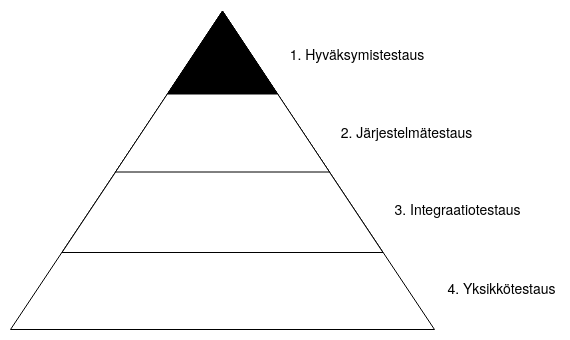
\includegraphics[width=0.8\textwidth]{assets/testauksen-tasot.png}
    \caption{Testauksen tasot pyramidin muodossa esitettynä.}
    \label{fig:testing-levels-pyramid}
  \end{figure}

  Kaikkiin pyramidimuodossa esitettyihin testauksen tasoihin on mahdollista soveltaa testiautomaatiota.
  Testauksen menetelmien osalta hieman yksinkertaistaen valkolaatikkotestauksen alaisuuteen kuuluvat yksikkötestaus ja integraatiotestaus sekä mustalaatikkotestauksen alaisuuteen kuuluvat järjestelmätestaus ja hyväksyntätestaus.
  Pyramidimuodossa alimpana kuvataan aina yksikkötestaus, joka on tasoista atomisin ja luo vahvan pohjan kokonaisvaltaiselle testaamiselle.
  Noustessa pyramidissa ylöspäin, atomisuus häviää ja testattavana olevan kohteen laajuus sekä kompleksisuus kasvavat.
  Ylimpänä pyramidissa on hyväksymistestaus, joka on tarkoituksellista toteuttaa vaatimusmäärittelyn täyttävää valmista järjestelmää vastaan siten, että sen varmistetaan vastaavan loppukäyttäjän tarpeita.
  Monissa tapauksissa järjestelmätestauksen ja hyväksymistestauksen rajat saattavat olla epäselvät ja häilyvät.
  Tässä työssä hyväksymistestauksella tarkoitetaan käyttäjän hyväksyttämistestausta, jotta järjestelmätestauksen ja hyväksymistestauksen väliset eroavaisuudet tulevat lukijalle selkeästi esille.

  Tämän diplomityön keskiössä on hyväksymistestaus, ja siihen liittyvää teoriaa esitetään vielä laajemmin omassa luvussaan.
  Seuraavissa kappaleissa esitetään vielä yksityiskohtaisemmin jokainen kuvassa \ref{fig:testing-levels-pyramid} esitetty testauksen taso, jotta lukijalle muodostuu käsitys erityisesti hyväksymistestauksen suhteesta muihin testauksen tasoihin.

  \subsection{Yksikkötestaus} \label{ch:07_yksikkotestaus}

    Yksikkötestaus on testauksen taso, joka keskittyy yksittäisten komponenttien, eli yksiköiden, testaamiseen.
    Yksikkötestauksen ajatuksena on siis testata ohjelmistotuotteen lähdekoodista löytyviä yksiköitä, kuten luokkia, komponentteja, funktioita tai moduuleita.
    Yksikkötestaus toteutetaan ohjelmiston toteuttavia pienimpiä yksikköjä vastaan ja sen avulla pyritään validoimaan, että jokainen yksikkö toimii siten kuin ne on ohjelmistokehityksen aloitusvaiheessa suunniteltu toimimaan.
    Yksikkötestausta hyödynnetään paljon myös testausvetoisen kehityksen aihepiirissä.
    Testausvetoisessa kehityksessä ohjelmistokehittäjät laativat yksikkötestit ennen yksiköiden toteuttamisen aloittamista.
    Yksikkötestaus eroaa muista testauksen tasoista siinä, että sen voivat suorittaa ainoastaan ohjelmistokehittäjät tai muut ohjelmiston lähdekoodiin perehtyneet henkilöt.
    Yksikkötestaus on näin ollen teknisesti ottaen valkolaatikkotestausta.
    Yksikkötestausta tarvitaan, jotta voidaan pyrkiä varmistamaan, että ohjelmiston koostavat pienimmät yksiköt toimivat tarkoituksenmukaisella tavalla. \cite{istqb_glossary_v3_3} \cite{testing_levels_webpage}

    Yksikkötestauksen toteuttamiseen käytetään pääsääntöisesti jotakin tarkoitusta varten räätälöityä testikirjastoa, joissa on keskenään yleensä hyvin samankaltainen perusperiaate.
    Yksikkötestaukseen tarkoitetuissa testikirjastoissa löytyy usein yksittäisen testitapauksen kuvaava tietorakenne, kuten luokka, sekä siihen usein kuuluvat alustus- ja lopetusfunktiot.
    Näiden lisäksi varsinainen testauskoodi toteutetaan pääsääntöisesti käyttäen niin sanottuja testikirjaston tarjoamia assert-funktioita, joiden avulla voidaan muun muassa varmistaa, onko jokin muuttuja tietyssä arvossa.

    Ohjelmistotestauksen tasojen pyramidissa ja hyvin toteutetussa ohjelmistotestauksen monitasoisessa testauksessa tämä testauksen taso on usein testitapauksien määrässä kaikista laajin.
    Monitasoisessa testauksessa yksikkötestaus luo tärkeän pohjan testaamiselle kokonaisuutena ja antaa tietoa ohjelmiston pienimpien yksiköiden toimivuudesta.
    Yksikkötestaus on myös paljon käytetty ja tärkeä osa testiautomaatiota, sillä se varmistaa sovelluksen yksiköiden suunniteltua toimintaa.

  \subsection{Integraatiotestaus} \label{ch:07_integraatiotestaus}

    Integraatiotestaus on testauksen taso, joka testaa rajapintoja ja vuorovaikutusta integroitavien yksiköiden välillä.
    Integraatiotestauksen ajatuksena on siis testata ohjelmistotuotteen toteuttavien eri komponenttien yhteensopivuutta niiden rajapintojen osalta.
    Integraatiotestaus toteutetaan ohjelmiston suunnitelmaa ja suunniteltua mallia vastaan.
    Integraatiotestauksen onnistunut toteuttaminen luo validoitavan perustan ohjelmiston toimimiseen ja sen koostamiseen kokonaisena, eri komponenteista koostuvana järjestelmänä.
    Integraatiotestausta tarvitaan, jotta voidaan varmistaa sovelluksen yksiköiden yhteensopivuus, joka ei pelkällä yksikkötestauksella tulisi muuten katetuksi. \cite{istqb_glossary_v3_3} \cite{testing_levels_webpage}

    Integraatiotestauksen kohteita voivat olla esimerkiksi luokkien ja moduulien väliset rajapinnat sekä web-sovelluksien API-ohjelmointirajapinnat.
    Integraatiotestauksen toteutuksen kannalta voidaan usein käyttää myös yksikkötestaukseen tarkoitettuja testikirjastoja ja -työkaluja, mutta itse testitapauksien rakenne on silloin yksikkötestauksen testitapauksista merkittävällä tavalla erilainen.
    Integraatiotestauksessa testitapauksien rakenteeseen tulee assert-funktioiden lisäksi myös usein tarve jäljitellä rajapintojen tarjoamaa dataa.
    Rajapintojen tarjoaman datan jäljittelemiseen on olemassa useita valmiita työkaluja ja kirjastoja, joita integraatiotestauksen tapauksessa voi käyttää testitapauksien rakentamisen apuna.

    Integraatiotestauksen yhteydessä puhutaan usein myös niin sanotusta savutestauksesta, jonka tarkoituksena integraatiotestauksen yhteydessä on koostaa toistuva, esimerkiksi päivittäinen, koontiversio ohjelmistosta ja testata sen kriittisten komponenttien yhteensopivuus \cite{testing_levels_webpage}.
    Integraatiotestaus on myös tärkeä osa testiautomaatiota, sillä sen avulla voidaan varmistaa sovelluksen yksiköiden, kuten esimerkiksi luokkien, komponenttien tai moduulien, yhteensopivuus.

  \subsection{Järjestelmätestaus} \label{ch:07_jarjestelmatestaus}

    Järjestelmätestaus on testauksen taso, joka keskittyy varmistamaan, että kokonainen järjestelmä vastaa sille asettuja vaatimuksia.
    Järjestelmätestauksen ajatuksena on siis testata kokonaista ja toimivaa järjestelmää yhtenä suurena yksikkönä.
    Järjestelmätestausta tarvitaan, jotta voidaan varmistaa kokonaisen ohjelmiston toimivuus, jota ei muuten pelkällä yksikkötestauksella ja integraatiotestauksella saataisi täydellisellä varmuudella selville.
    Järjestelmätestaukseen liittyy laajasti erilaisia testattavia laadullisia ominaisuuksia, kuten toiminnallisuus, luotettavuus, käytettävyys, tehokkuus, ylläpidettävyys ja siirrettävyys \cite{iso_quality_attributes}.
    Aiemmin testiautomaation tarkoitus kappaleessa esitettiin että edellä mainituista laadullisista ominaisuuksista kaikki eivät sovellu hyvin testiautomaation avulla testattaviksi.
    Esitetyistä syistä johtuen, automatisoidulla järjestelmätestauksella voidaan testata edellä mainituista ominaisuuksista lähinnä ohjelmiston toiminnallisuutta, luotettavuutta ja tehokkuutta.
    Toiminnallisuutta voidaan testata käyttöliittymätestauksella, joka on mahdollista automatisoida käyttötapauksien muotoon.
    Luotettavuutta voidaan testata automaattisesti tietoturvaa testaavien käyttötapauksien muodossa.
    Tehokkuutta voidaan testata automaattisesti lisäämällä aikaleimoihin perustuvaa tarkastelua testitapauksiin, sekä tekemällä kuormitusta testaavia testitapauksia.
    Edellä mainituista muista laadullisista ominaisuuksista voidaan kuitenkin ylläpidettävyyttä ja siirrettävyyttä testata myös manuaalisesti. \cite{istqb_glossary_v3_3} \cite{testing_levels_webpage}

    Testauksen tasona järjestelmätestaus voi olla testiautomaation teknisen toteutuksen kannalta jopa hyvin samanlainen kuin sitä kapeampi hyväksymistestaus.
    Usein kuitenkin hyväksymistestauksessa paneudutaan erityisesti vaatimusmäärittelyyn ja asiakaslähtöiseen testaamiseen, kun taas järjestelmätestauksessa voidaan testata myös esimerkiksi järjestelmän tehokkuutta tai tietoturvaa.
    Tämä on tosin täysin riippuvainen vaatimusmäärittelystä, joten jos tehokkuus ja tietoturva ovat ohjelmiston asiakasvaatimuksia, niin niiltä osin järjestelmätestaus ja hyväksymistestaus lomittuvat.
    Joissakin yhteyksissä järjestelmätestaus ja hyväksymistestaus esitetään jopa yhteisenä testauksen tasona, etenkin silloin kun testiautomaation kannalta ne esimerkiksi edellä mainitulla tavalla muistuttavat kovasti toisiaan.
    Järjestelmätestaus osittain hyväksymistestauksen kanssa on erittäin merkittävä osa testiautomaatiosta, sillä sen avulla voidaan testata toteutettavaa järjestelmää kokonaisuutena.

  \subsection{Hyväksymistestaus} \label{ch:07_hyvaksymistestaus}

    Hyväksymistestaus on testauksen taso, joka keskittyy selvittämään voidaanko järjestelmä hyväksyä.
    Hyväksymistestauksen ajatuksena on varmistaa toteutettavan ohjelmiston vaatimusten toimivuus erityisesti käytännön tilanteissa siten, että voidaan varmistaa, vastaako ohjelmisto loppukäyttäjän tarpeita.
    Hyväksymistestaus toteutetaan ohjelmiston toimintoja kuvaavaa vaatimusmäärittelyä tai loppukäyttäjistä sekä heidän tarpeista laadittuja käyttötapauksia vastaan.
    Hyväksymistestauksen rooli testiautomaatiossa ja erityisesti jatkuvan integraation yhteydessä on osoittaa, voidaanko järjestelmä julkaista sellaisenaan loppukäyttäjille. \cite{istqb_glossary_v3_3} \cite[s.~373]{software_testing_book}

    Hyväksymistestauksen avulla voidaan testata erityisesti toiminnallisia laatuominaisuuksia, jotka usein toteutetaan käyttöliittymätasolla testitapauksien muodossa.
    Toiminnallisten ominaisuuksien lisäksi hyväksymistestauksessa voi olla mukana myös muita laadullisia ominaisuuksia, jos ne ovat asiakastarpeiden mukaisia.
    Samassa asiayhteydessä puhutaan usein myös niin sanotusta e2e-testauksesta, eli päästä päähän -testauksesta.
    Päästä päähän -testauksessa on tarkoituksena toteuttaa testaaminen siten, että testaus pitää sisällään kaiken siltä väliltä, mitä loppukäyttäjä voi tarpeidensa saavuttamiseksi tehdä ja nähdä aloittaessaan ohjelmiston käytön ja lopettaessaan sen käytön.

    Testiautomaatio on äärimmäisen hyödyllinen hyväksymistestauksen tasolla, koska sillä voidaan automatisoida ohjelmiston validointi ja hyväksyminen, sekä parhaimmillaan estää puutteellisesti toimivan ohjelmiston julkaiseminen.
    Hyväksymistestausta tarvitaan myös, jotta voidaan testata ja validoida vaatimusten ja loppukäyttäjän tarpeiden mukaisten ominaisuuksien toimivuus kokonaisessa järjestelmässä.

\section{Testitapaukset ja testikokoelmat} \label{ch:07_testitapaukset_ja_testikokoelmat}

  Testitapaus on ohjelmistotestauksen automatisoimisen kannalta erittäin tärkeä käsite, joka koostuu ohjelmistolle annettavista syötteistä ja oletetusta ulostulosta \cite[s.~21]{software_testing_book}.
  Testitapaus kuvaa yhden testattavana olevan asian testaamiseksi suoritettavaa tai suoritettavia toimenpiteitä.
  Testitapauksen sisältämien toimenpiteiden suorittamisen tarkoituksena on saada selville, täyttääkö se toimenpiteiden mukaiset ehdot, ja toimiiko testattava asia oikein.
  Testitapauksella on usein kolme vaihetta: alustusvaihe, varsinainen testausvaihe ja lopetusvaihe.
  Alustusvaiheessa testitapauksen vaativa ympäristö ja muuttujat alustetaan.
  Varsinaisessa testitapauksen testausvaiheessa suoritetaan testattavan asian testaukseen liittyvät toimenpiteet.
  Lopetusvaiheessa testitapauksen ajaksi muodostettu ympäristö usein tuhotaan ja käytetyt resurssit nollataan, jotta ne eivät enää vaikuta muihin testitapauksiin.

  Testikokoelma on yksittäisistä testitapauksista koostuva ryhmitelty testitapauksien joukko \cite[s.~22]{software_testing_book}.
  Testikokoelmaan saattaa kuulua myös sellaisia testitapauksia, joiden suoritusjärjestys on etukäteen määritetty.
  Suoritusjärjestyksellisissä testikokoelmissa voi esiintyä testitapauksia, jotka toimivat samassa testausympäristössä muokaten ja jättäen jälkiä omasta suorituksestaan.
  Myöhemmin suoritusjärjestyksessä tulevat testitapaukset voivat siinä tapauksessa hyödyntää tai vaatia testausympäristön ominaisuuksia, jotka aiemmat testitapaukset ovat asettaneet.
  Testikokoelman sisältämät testitapaukset voidaan kuitenkin luonnollisesti laatia myös sellaisella tavalla, että jokainen testitapaus hoitaa yksityiskohtaiset alustustoimenpiteensä itsenäisesti.

  Testitapauksia voidaan ryhmitellä samaan kontekstiin liittyviksi testikokoelmiksi tilanteesta riippuen monin eri tavoin.
  Ryhmittelyn perusteen valitsemiseen kannattaa käyttää harkintaa, sillä testikokoelmien laajuus on helpomman hallittavuuden takia tärkeää.
  Yksi tapa ryhmitellä testitapauksia on käyttää ryhmittelyn perustana ohjelmistojen laadullisia ominaisuuksia.
  Tällaisessa ryhmittelyssä yksi kokoelma voi olla toiminnallisille testitapauksille ja toinen tehokkuutta mittaaville testitapauksille.
  Laadullisten ominaisuuksien mukaan tehty testitapauksien ryhmittely saattaa kuitenkin johtaa määrällisesti liian suuriin testitapauksien eroihin testikokoelmien kesken.
  Hyväksymistestauksen näkökulmasta tarkasteltuna testitapauksia on mahdollista ryhmitellä käyttöliittymän näkymiin perustuviin testikokoelmiin.
  Näkymäperusteinen ryhmittely on osaltaan looginen tapa jakaa testitapaukset eri testikokoelmiin, sillä jokainen käyttöliittymän näkymä voidaan tarvittaessa testata erikseen suorittamalla kyseisen testikokoelman testitapaukset.
  Tässä diplomityössä hyödynnetään perustavanlaatuisesti näkymäperusteista testitapauksien ryhmittelyä, koska sen avulla on mahdollista suorittaa testikokoelmien näkymäperusteinen priorisointi työssä myöhemmin esitettävää painotettua verkkoa hyödyntäen.

\section{Jatkuva integrointi} \label{ch:07_jatkuva_integrointi}

  Testiautomaation rakentaminen manuaalisen testaamisen sijaan mahdollistaa sen liittämisen osaksi jatkuvaa integrointia.
  Lisäksi useissa ohjelmistotuotannon prosesseissa pelkkä manuaalinen testaus kävisi selkeästi automatisoitujen koonti- tai julkaisuputkien periaatteita vastaan.
  Testiautomaation tarkoitusta käsittelevässä kappaleessa esitettiin testiautomaation ja manuaalisen testauksen eroja hyötyjen ja haittojen näkökulmasta.
  Testiautomaation toteuttaminen testitapauksien muodossa on jo itsessään testiautomaatiota, mutta käsitettä voidaan kuitenkin laajentaa, että myös jatkuva integrointi liittyy oleellisesti testiautomaation toteuttamiseen varsinkin nykyaikana ja erityisesti ketteriin menetelmiin painottuvassa ohjelmistokehityksessä \cite{agile_testing_book}.

  Jatkuva integrointi tarkoittaa sellaista ohjelmistojen kehitystapaa, joka vaatii ohjelmistokehittäjiä integroimaan koodimuutokset jaettuun repositorioon useita kertoja päivässä.
  Tämän lisäksi jokainen koodimuutos verifioidaan automatisoidun koontiversion avulla, jolloin kehitystiimi huomaa mahdolliset ongelmat mahdollisimman aikaisin. \cite[s.~23]{devops_for_web_book}
  Toisin sanoen jatkuvalla integroinnilla tarkoitetaan versiohallintaisessa ohjelmistokehityksessä väistämättömän integrointiprosessin muuntamista luonnostaan jatkuvaksi.
  Ohjelmistokehityksessä integrointiprosessi tulee siis vastaan, kun eri ohjelmistokehittäjät tai tiimit toteuttavat muutoksia tai uusia ominaisuuksia kehitettävänä olevaan ohjelmistotuotteeseen.
  Tällaisessa tilanteessa yksittäiset ohjelmistokehittäjät tai tiimit toteuttavat uutta ohjelmakoodia toisistaan irrallaan siihen asti, kunnes muutokset tai ominaisuudet tulee yhdistää yhdeksi kokonaiseksi kehityksen kohteena olevaksi ohjelmistotuotteeksi.
  Tätä prosessia kutsutaan integrointiprosessiksi.
  Jatkuvan integroinnin tarkoituksena on nopeuttaa integrointiprosessia ja muuttaa ohjelmistokehityksessä käytössä olevia periaatteita siten, että siitä tulee jatkuvaa.
  Jatkuvan integroinnin toteuttaminen tarvitsee teknisesti sen mahdollistavan versionhallintajärjestelmän ja varsinaisen jatkuvan integroinnin palvelimen, kuten kuvassa \ref{fig:jatkuva-integrointi} esitetään.

  \begin{figure}[H]
    \centering
    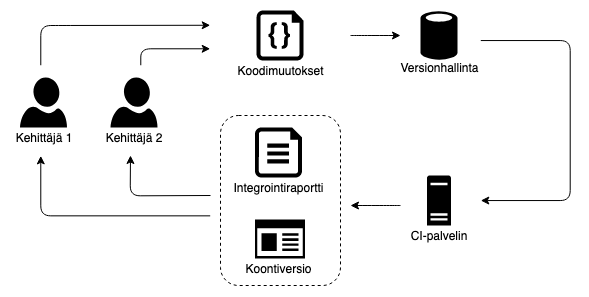
\includegraphics[width=0.8\textwidth]{assets/jatkuva-integrointi.png}
    \caption{Jatkuvan integroinnin perusperiaate on iteratiivinen.}
    \label{fig:jatkuva-integrointi}
  \end{figure}

  Esimerkkinä ver\-si\-on\-hal\-lin\-ta\-jär\-jes\-tel\-mä\-stä  voidaan käyttää nykyaikana suosittua git-oh\-jel\-mis\-to\-a  ja jatkuvan integroinnin palvelimena esimerkiksi GoCD-oh\-jel\-mis\-to\-a.
  Perusideana jatkuvassa integroinnissa on konfiguroida jatkuvan integraation mahdollistava palvelinohjelmisto siten, että se kuuntelee versionhallintaan tulevia muutoksia, ja suorittaa integrointiprosessin jatkuvasti aina muutoksia huomattuaan.
  Versionhallintaan tulevat muutokset voidaan jatkuvan integraation osalta kuunnella ajastetusti tietyin väliajoin tai aidosti jatkuvalla tavalla käyttämällä esimerkiksi web-koukkuja, jotka tiedottavat jatkuvan integraation palvelimelle versionhallintaan saapuneista muutoksista \cite{github_webhooks}.
  Jatkuvassa integroinnissa yhden iteraatiokerran integrointiprosessin lopputuloksen on tarkoitus tarjota periaatteeltaan sama lopputulos, kuin mitä se olisi manuaalisella integrointiprosessilla.
  Jatkuvan integroinnin mahdollistava konfiguraatio sisältää aina jonkinlaisen koontiputken tai useita koontiputkia, joissa rakennetaan koontiversio kehitettävän ohjelmiston lähdekoodeista.
  Koontiputki voi sisältää esimerkiksi ohjelman lähdekoodien kääntämisen asiaan sopivalla kääntäjällä.
  Kääntämisen lisäksi koontiputkeen on tässä vaiheessa mahdollista ja erittäin kannattavaa yhdistää testiautomaatiota, kuten esimerkiksi automaattisten yksikkötestien suorittaminen ennen kääntämistä ja hyväksymistestien suorittaminen valmiille koontiversiolle kääntämisen jälkeen.

  Jatkuvan integroinnin yhteydessä suoritettavat testikokoelmat ja niiden sisältävät testitapaukset ovat erittäin järkeviä toteuttaa, sillä ne muun muassa parantavat ohjelmistokehityksen ja lopputuotteen luotettavuutta ja laatua.
  Jatkuvan integroinnin sisältämästä koontiputkesta saadaan hyödyllistä palautetta ja raportteja integrointiprosessin onnistumisesta, joka voidaan ohjata pääasiassa ohjelmistokehittäjille sekä myös muillekin sidosryhmille.
  Jatkuvalla integroinnilla itsessään on myös paljon sen käyttöönoton antamia hyötyjä, kuten esimerkiksi toteutettujen muutosten tai toimintojen integrointitiheyden kasvattamisen tuomat edut.
  Jos muutosten tai toimintojen integroiminen on perinteisessä ohjelmistokehityksessä tehty harvoin, kuten esimerkiksi kerran viikossa, niin jatkuva integroiminen korjaa sen tuomat haasteet turhan laajasta integrointiprosessista ja mahdollisesta ohjelmistokoodin hajoamisesta.
  Tällaisissa tapauksissa ohjelmakoodi voi sisältää epäyhteensopivia moduuleita tai muita rajapintoja, sekä mahdollisuuden käännettävien lähdekoodien kääntämisen onnistumisesta.

\section{Testausvetoinen kehitys} \label{ch:07_testausvetoinen_kehitys}

  Perinteisesti testiautomaatio on soveltunut hyvin vain valmiille ohjelmistoille ja niiden regressiotestaamiseen.
  Nykypäivänä ohjelmistokehitys on kuitenkin yhä enemmän siirtynyt suunnitelmapohjaisista prosesseista iteroiviin ja ketteriin ohjelmistotuotannon prosesseihin.
  Testiautomaatio on soveltunut näihin huonosti siksi, että testattavaa ohjelmistoa tai lisättyä toiminnallisuutta ei ole vielä ollut olemassa.
  Tähän ongelmaan on kehittynyt niin sanottu testausvetoinen kehitys, jossa testitapaukset suunnitellaan ja toteutetaan läpäistäkseen testitapaukset ennen varsinaisen ohjelmiston tai toiminnon inkrementiaalista toteuttamista \cite{istqb_glossary_v3_3}.

  \begin{figure}[H]
    \centering
    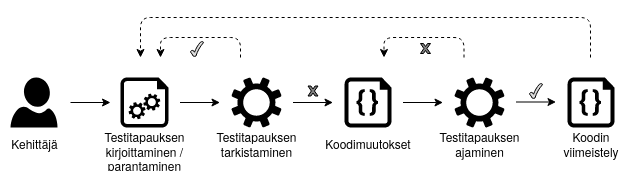
\includegraphics[width=0.8\textwidth]{assets/testausvetoinen-kehitys.png}
    \caption{Testausvetoisen kehityksen vaiheet \cite[s.~2]{tdd_paper}.}
    \label{fig:testausvetoinen-kehitys}
  \end{figure}

  Testausvetoinen kehityksen sisältämät vaiheet on esitetty kuvassa \ref{fig:testausvetoinen-kehitys}, jossa ne alkavat testitapauksien luomisesta ja niiden tarkastamisesta.
  Tarkastaminen tapahtuu siten, että testitapaukset suoritetaan sillä oletuksella, että niiden täytyy tässä vaiheessa epäonnistua.
  Alkuvaiheen testitapauksien luomisen jälkeen ohjelmistokehittäjät kehittävät ohjelmistoa tekemällä siihen muutoksia, ihanteellisesti testitapauksien kokoisia paloja kerrallaan.
  Kun koodimuutoksia on syntynyt, ohjelmistotuotannossa käytössä olevasta integrointiprosessista riippuen testitapaukset ajetaan joko manuaalisesti tai jatkuvan integroinnin avulla.
  Integrointiprosessista saadaan palautetta, jonka mukaan ohjelmakoodia korjataan tai viimeistellään.
  Testausvetoisella kehityksellä pyritään nopeuttamaan ohjelmistokehitysprosessia perinteisiin ohjelmistotuotannon menetelmiin verrattuna.
  Tämän jälkeen testausvetoista kehitystä käyttävässä ohjelmistotuotantoprosessissa siirrytään takaisin testitapauksien luomiseen ja parantamiseen, sekä aloitetaan toinen iteraatiokierros, mikäli ohjelmisto ei vielä ole valmis. \cite{tdd_paper}

  Testausvetoisessa kehityksessä testitapaukset siis laaditaan jo varhaisessa vaiheessa, jolloin niiden tekeminen saattaa usein olla liiketoiminnan näkökulmasta helpommin perusteltavissa liiketoiminnan johdolle.
  Tämän lisäksi testitapauksien kirjoittaminen etukäteen luo alusta alkaen kattavat testikokoelmat, joita voidaan hyödyntää iteratiivisesti ohjelmistotuotteesta riippuen usein hyvinkin pitkään, etenkin jos niihin tehdään tarvittavaa hienosäätöä ohjelmistokehityksen aikana.
  Ohjelmistokehittäjät voivat kehittää helposti hallittavissa olevia testitapauksia rajaavia kokonaisuuksia, jolloin ohjelmistotuote valmistuu ikään kuin pala kerrallaan.
  Itse ohjelmistokehitys on testausvetoisessa kehityksessä iteratiivista ja näin ollen testitapauksien suorittamisesta saadaan palautetta ja raportointia koko ohjelmistotuotantoprosessin ajan.

\chapter{Hyväksymistestaus} \label{ch:08_hyvaksymistestaus}
  Tässä luvussa esitetään perusteet ja tarvittavat tiedot hyväksymistestauksesta, johon testauksen tasoista tässä diplomityössä keskitytään.
Ensin esitetään hyväksymistestauksen tarkoitus, jonka jälkeen keskitytään hyväksymistestausvetoiseen kehitykseen ja sen esittelemiseen ohjelmistotuotannollisena menetelmänä.
Hyväksymistestausvetoisen kehityksen jälkeen käydään läpi tässä diplomityössä käytettyä ja lähes de facto testialustaa, Robot frameworkia, hyväksymistestauksen testitapauksien rakentamiseen.
Robot frameworkin perusteiden jälkeen esitetään hyväksymistestauksen testitapauksien laatiminen käyttäen Robot frameworkia sekä esitetään web-sovelluksien erityispiirteitä jotka on huomioitava hyväksymistestauksessa.
Hyväksymistestaksen perusteiden ymmärtämistä tarvitaan työn toteutusvaiheessa, jossa esitetään korkealla tasolla asiakasyritykselle toteutettua hyväksymistestausta ja sen automaatiota.
Lopuksi esitetään yleisestikin ottaen testitapauksiin tärkeästi liittyvä priorisointiongelma ja käydään läpi sen eri ratkaisumalleja, keskittyen erityisesti tässä diplomityössä myöhemmin esitettävään priorisointiin painotetun verkon avulla.

\section{Hyväksymistestauksen tarkoitus} \label{ch:08_hyvaksymistestauksen_tarkoitus}

  Hyväksymistestauksen tarkoituksena on varmistaa toteutettavan ohjelmiston vaatimusten toimivuus erityisesti käytännön tilanteissa siten, että voidaan varmistaa vastaako ohjelmisto loppukäyttäjän tarpeita.
  Hyväksymistestaus antaa vastauksen siihen, toimiiko toteutettu järjestelmä loppukäyttäjän tarpeiden mukaisesti ja loppukäyttäjän näkökulmasta oikein.
  Hyväksymistestauksen sanotaan olevan muodollista testaamista, jossa käyttäjän tarpeet, vaatimukset ja liiketoimintaprosessit otetaan huomioon selvittäessä täyttääkö järjestelmä hyväksymisen kriteerit ja sallii käyttäjän, asikkaiden tai muun autorisoidun tahon päättää hyväksytäänkö järjestelmä \parencite{istqb_glossary_nodate}.
  Ohjelmistotestauksen tekniikoiden näkökulmasta hyväksymistestaus on mustalaatikkotestausta, eli sitä testataan tietämättä sen teknisestä toteutuksesta.
  Hyväksymistestauksen painoarvo on asiakaperusteisessa vaatimusmäärittelyssä ja loppukäyttäjän tarpeiden kartoittamisessa.
  Testiautomaation osalta hyväksymistestausta varten voidaan rakentaa testitapaukset, joiden avulla voidaan keskittyä varmistamaan loppukäyttäjille tarpeellisten toimintojen toteutuminen testitapauksien suorittamisen jälkeen.
  Hyväksymistestauksen osalta testitapauksia voidaan toteuttaa niin sanotulla päästä päähän -periaatteella, jossa testattavaa järjestlemää testataan siten kuin loppukäyttäjä sitä käyttää.
  Hyväksymistestauksessa ei anneta suurta painoarvoa kosmeettisille tai kirjoitusvirheille, vaan pyritään selvittämään loppukäyttäjille oleellisten ja tarpeellisten toimintojen toteutuminen.

  Hyväksymistestaus on aiemmin esitetyistä testauksen tasoista \ref{ch:07_testauksen_tasot} viimeinen ja sen suorittamisen jälkeen saadaan tieto siitä onko järjestlemä toteutuksen osalta sellaisenaan valmis julkaistavaksi.
  Perinteisesti hyväksymistestauksen lähtökohtia ovat selvät hyväksymisvaatimukset sekä julkaisukelpoinen toteutus joka voi sisältää vain kosmeettisia virheitä.
  Hyväksymisvaatimukset voivat olla esimerkiksi liiketoiminnallisia käyttötapauksia, prosessivirtauskaavioita sekä ohjelmiston vaatimusmäärittely.
  Testiautomaatiota varten käytettävästä testialustasta riippuen hyväksymistestauksen käyttötapaukset voidaan muodostaa joko osittain tai suoraan testitapauksiksi.
  Hyväksymistestaukseen usein osallistuu ohjelmistokehittäjien lisäksi myös muut sidosryhmät ja loppukäyttäjät.
  Keskeistä on, että loppukäyttäjiltä hankitaan tieto tarvittavista ja toteutettavista ominaisuuksista, kun taas muut sidosryhmät kuten esimerkiksi johtoryhmä voivat tehdä liiketoiminnallisia päätöksiä hyväksymistestauksen onnistumisen osalta ja esimerkiksi peruuttaa julkaisun.
  Hyväksymistestaus antaa mahdollisuuden korjata usein liiketoiminnalisestakin näkökulmasta merkittävät toiminalliset virheet ennen järjestelmän julkaisua loppukäyttäjille.

  Kehittäjien käsitys järjestelmän toiminnallisuudesta ja sen vaatimuksista voi olla usein hyvinkin erilainen kuin loppukäyttäjien.
  Hyväksymistestauksen avulla voidaan tätä lievittää tätä ongelmaa, ja saattaa ohjelmistokehittäjät loppukäyttäjien kanssa vaatimusmäärittelyn suhteen samalle sivulle.
  Testiautomaation avulla toteutettavalla toistuvalla hyväksymistestauksella varmistetaan, että järjestelmä toteuttaa loppukäyttäjän tarpeet vielä järjestlemään tehtyjen muutoksien jälkeenkin.
  Hyväksysmistestauksen testitapaukset tarkoituksenmukaisesti heijastavat suoraan loppykäyttäjien tarpeita, joka on iso etu sillä sen avulla ohjelmistokehittäjät ja muut sidosryhmät voivat tehokkaasti varmistaa järjestlemän valmiuden ja tilan.
  Hyväksymistestauksella siis saadaan katsaus ohjelmiston valmiudesta sen vaatimuksiin ja loppukäyttäjien toiminnallisiin tarpeisiin nähden.

\section{Hyväksymistestausvetoinen kehitys} \label{ch:08_hyvaksymistestausvetoinen_kehitys}

  Hyväksymistestausvetoisen kehityksen (englanniksi: ATDD, acceptance test driven development) tarkoituksena, kuten testausvetoisessakin kehityksessä \ref{ch:07_testausvetoinen_kehitys} on toteuttaa ohjelmistotuotannollinen prosessi laatien toistettavasti suoritettavat testitapaukset ennen ohjelmiston varsinaista toteutusta.
  Hyväksymistestausvetoisessa kehityksessä tämä tarkoittaa käytännössä sitä, että ennen toteutusta luodaan tarvittavat ohjelmiston asiakasvaatimuksia palvelevat hyväksymistestit, jotka ohjelmiston on tarkoitus läpäistä sen julkaisemisen hyväksymiseksi.
  Hyväksymistestausvetoisen kehityksen sanotaan olevan yhteistyöhön perustuva lähestymistapa kehitykseen, jossa tiimi ja asiakkaat käyttävät asiakkaiden oman ympäristön kieltä ymmärtääkseen heidän vaatimukset, jotka muodostavat pohjan komponentin tai järjestelmän testaamiseen \parencite{istqb_glossary_nodate}.
  Tarvittavat ohjelmiston hyväksymistestit suoritetaan iteratiivisesti ohjelmistokehitysprosessin aikana ja se tarkoittaa käytännössä jatkuvan integraation \ref{ch:07_jatkuva_integrointi} ottamista käyttöön ohjelmistokehityksessä.
  Hyväksysmistestausvetoinen kehitys on erittäin hyödyllinen ohjelmistokehityksessä käytetty menetelmä, sillä kehitysvaiheessa on aina tarkasti tiedossa vastaako ohjelmiston tila asiakasvaatimuksia ja kuinka hyvin se niiden täyttämisessä onnistuu.

  \begin{figure}[H]
    \centering
    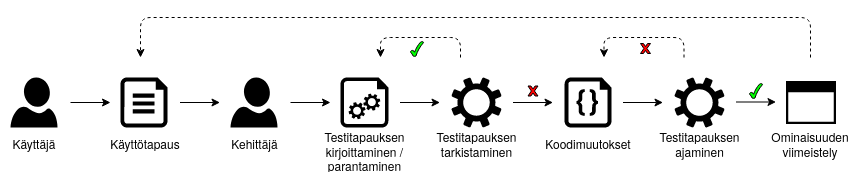
\includegraphics[width=0.8\textwidth]{assets/hyvaksymistestausvetoinen-kehitys.png}
    \caption{Hyväksymistestausvetoisen kehityksen vaiheet}
    \label{fig:hyvaksymistestausvetoinen-kehitys}
  \end{figure}

  Hyväksymistestausvetoinen kehitys voidaan luokitella ketteräksi ohjelmistokehitysmenetelmäksi, kuten sen yläkäsitteenä oleva testausvetoinen kehityskin \ref{ch:07_testausvetoinen_kehitys}.
  Hyväksymistestausvetoinen kehitys on testausvetoisen kehityksen kanssa perusperiaatteeltaan samanlainen, mutta ennen ohjelmistokehityksen aloitusta asiakasvaatimukset kartoitetaan ja ohjelmiston hyväksyttävyys määritetään.
  Hyväksymistestitapaukset kirjoitetaan testausvetoisen kehityksen mukaisesti ensin ja ohjelmistokehitys itsessään noudattaa iteratiivisesti testausvetoista kehitystä, vaikkakin hyväksymistestaus itsessään on perinteisesti vaatinut lähes valmista järjestlemää.
  Asiakasvaatimukset määritetään usein käyttötapauksien muotoon, ja riippuen testialustasta ne voidaan kirjottaa testitapauksien muotoon niitä vahvasti hyödyntäen.
  Hyväksymistestausvetoisessa kehityksessä ohjelmistokehitystä siis ohjaavat asiakasvaatimukset ja loppukäyttäjien tarpeiden toteutuminen, jotka ovat hyvin usein toiminallisia vaatimuksia.
  Hyväksymistestausvetoisessa kehityksessä mitataan jatkuvasti iteroiden käyttötapauksien muodossa validoitavien haluttujen ominaisuuksien toteutumista.
  Perusperiaate on kirjoittaa asiakasvaatimus tai käyttötapaus testitapauksen muotoon, toteuttaa testitapaus, ajaa testitapaus läpäisemättömänä, toteuttaa ominaisuus, ajaa testitapaus läpäisevänä, refaktoroida toteutus ja siirtyä takaisin seuraavaan käyttötapaukseen.
  Käyttötapaus koostuu rakenteellisesti usein tilanteesta, motivaatiosta ja halutusta lopputuloksesta.
  Esimerkki käyttötapauksesta voi olla: \emph{käyttäjänä, haluan sisäänkirjautumisen jälkeen voida avata premium ominaisuudet tekemällä sovelluksensisäisen oston}.

  Hyväksymistestausvetoisessa kehityksessä hyväksymistestit on hyödyllistä pilkkoa pieniin hallittaviin kokonaisuuksiin, jolloin voidaan iteratiivisesti toteuttaa valmiiksi tietyn testitapauksen mukainen ominaisuus, joka vastaa jotakin käyttötapausta tai loppukäyttäjän tarvetta.
  Hyväksymistestauksessa testitapaus voi olla esimerkiksi käyttäjän tietojen muuttuminen varmistaminen, kuten tason läpäiseminen pelisovelluksessa, joka muuttaa käyttäjän edistystä.
  Hyväksymistestausvetoisen kehityksen tarkoituksena menetelmänä on onnistua vastaamaan loppykäyttäjän tarpeisiin tehokkaasti ja hyvin ottamalla tarpeet huomioon jo ennen toteutuksen aloittamista.
  Menetelmän avulla myös luodaan ymmärrystä ohjelmistotuotteen valmiuden määritelmästä kun eri sidosryhmän voidaan saada sen suhteen samalle aaltopituudelle.
  Hyväksymistestausvetoinen kehitys on lisäksi erittäin hyödyllistä, sillä jatkuva testaaminen antaa mahdollisuuden haluttujen ominaisuuksien toteutumisen validoimiselle menetelmän jokaisen iteraation koontiversiossa.

\section{Web-sovelluksien erityispiirteet} \label{ch:08_websovelluksien_erityispiirteet}

  Web-sovelluksilla on omia erityispiirteitä, jotka vaikuttavat testitapauksien laatimiseen.
  Nykypäivänä web-sovellukset ovat kasvaneet kompleksisuudessa ja front-end puolen toteutuksesta tarkasteltuna web-sovellukset usein muistuttavat jo perinteisiä työpöytäsovelluksia.
  Web-sovelluksia päivitetään nykyään tiheään tahtiin ja niille on suuri tarve luoda testiautomaatiota, jota hyödyntäen voidaan varmistaa että ne toimivat oikein muutoksien jälkeenkin.

  Hyväksymistestauksen priorisoimisen osalta tärkeä web-sovelluksien erityispiirre liittyy käyttöliittymiin ja dokumenttiobjektimalliin, DOM.
  Dokumenttiobjektimallin avulla verkkoselaimet renderöivät käyttöliittymän ja siinä näkyvän sisällön.
  Tämän lisäksi dokumenttiobjektimalli mahdollistaa käyttöliittymässä olevien elementtien valitsemisen, jota hyödynnetään myös testitapauksien kirjoittamisessa.

  Navigointi ja navigointiketjut ovat myös yksi web-sovelluksien erityispiirre.
  Historiallisesti verkkosivuilla navigointi tapahtui niin kutsuttujen hyperlinkkien avulla, verkkosivujen itse ollessa hypertekstiä.
  Tämä historiallinen lähestymistapa on edelleen käytössä ja web-sovelluksissa on lähes poikkeuksetta useita hyperlinkkejä joiden avulla navigoiminen luo erityisiä navigointiketjuja, joissa edelliseen sivuun tiedetään palata.
  Hyperlinkkien avulla tapahtuva navigointi ja navigointiketjut on erityispiirre, joka on hyvä tiedostaa myös hyväksymistestauksen testitapauksia rakentaessa.

  Web-sovelluksien syötteet ja niiden yhteyteen liittyvä tietoturva ovat myös yksi niiden erityispiirre joka vaatii suurta huomiota.
  Web-sovelluksien syötteisiin on perinteisesti liittynyt paljon haavoittuvuuksia, kuten esimerkiksi XSS-hyökkäykset ja SQL-injektiot.
  Web-sovelluksien hyväksymistestauksen testitapauksiin on hyvä sisällyttää syötteisiin liittyvää testaamista, joissa tietoturva pidetään mielessä.

  Erilaisia web-sovelluksen loppukäyttäjien asiakasympäristöjä on huikean paljon, joka kannustaa moniselaimellisen testauksen rakentamiseen.
  Näissä ympäristöissä on omat verkkoselaimensa, näyttöresoluutio ja selainasetukset, jotka saavat saman sovelluksen toimimaan eri tavoilla eri ympäristöissä ja luovat siten usein jopa päänvaivaa ohjelmistokehittäjille.
  Etenkin web-käyttöliittymiin keskittyessä testitapauksiin on hyvä sisällyttää erilaisia näyttöresoluutioita, kuvankaappauksien ottamista ja selainasetuksista esimerkiksi Javascript-ominaisuuksien estäminen.

  Web-sovelluksien käyttöliittymien testaaminen ja yleisestikkin ottaen käyttöliittymien testaaminen on perinteisesti tapahtunut manuaalisesti.
  Nykyään web-sovelluksia voidaan testata niin sanotun päätteettömän testauksen keinoin.
  Web-sovelluksien päätteettömässä testauksessa verkkoselaimen, näyttöresoluution ja selainasetuksien muodostamaa asiakasympäristö rakennetaan virtualisoinnin avulla.
  Virtualisoinnista vastaa joko verkkoselain itse tai voidaan käyttää UNIX järjestelmissä x-näyttöpalvelimen protokollan toteuttavaa virtualisointiratkaisua, esimerkiksi Xvfb.
  Virtualisoitu asiakasympäristö rakennetaan siten, että se päätteettömänä vastaa täysin päätteellistä vaihtoehtoa, ja siitä voidaan ottaa esimerkiksi kuvankaappaus vaikka mitään ihmisen astittavaa ei ole näkyvillä.

\section{Hyväksymistestauksen työkaluja} \label{ch:08_hyvaksymistestauksen_tyokaluja}

  Tässä kappaleessa esitetään diplomityötä tehdessä käytettyjä ja osin myös varsin yleisiä testiautomaation mahdollistavia työkaluja, kukin omassa alikappaleessaan.
  Ensin esitetään hyväksymistestauksen automatisoimisen kannalta kaikista tärkeimmät työkalut, eli testikehyksenä käytettävä Robot framework ja web-sovelluksien interaktioiden automatisoimisen mahdollistava Selenium kirjasto.
  Lisäksi esitetään kolme muuta tärkeää työkalua joiden avulla voidaan rakentaa kokonainen ohjelmistotuotannon prosessiin intergroitavissa oleva hyväksymistestausjärjestelmä.
  Toteutuksessa GoCD vastaa jatkuvan integroinnin tarjoamisesta, Xvfb vastaa päätteettömän testauksen tarjoamisesta ja Docker vastaa työkalujen virtualisoimisesta ja säiliöinnistä, jolloin työkaluista saadaan luotua yhtenäinen kokonaisuus.

  \subsection{Robot Framework} \label{ch:08_robot_framework}

    Robot framework on geneerinen avoimen lähdekoodin testausalusta hyväksymistestaukseen, hyväksymistestausvetoiseen kehitykseen ja robotisten prosessien automaatioon \parencite{noauthor_robot_nodate}.
    Testialustana Robot frameworkilla on helposti ymmärrettävä, luettava ja selkeä avainsanaperustainen syntaksi.
    Testialustan etuna on helppo lähestyttävyys ja sen pohjalle rakennettujen testitapauksien ymmärtäminen ei vaadi ohjelmakoodin ymmärtämistä.
    Robot framework on Python-perustainen testialusta joka on helppo asentaa, sitä on helppoa ymmärtää, sillä on kattava dokumentaatio ja se on helppoa ottaa käyttöön.

    Robot frameworkissa on sisäänrakennettu tuki ulkoisille kirjastoille ja dokumentaatiosta löytyy paljon tietoa omien avainsanojen ja omien kirjastojen tekemiseen.
    Lisäksi Robot framework on todella suosittu ja sisäänrakennettujen ominaisuuksien lisäksi ulkoisia kolmansien osapuolien kirjastoja löytyy alustalle paljon.
    Robot framework tukee muuttujien käyttöä testitapauksien rakentamisessa, joilla voi lisätä hieman kompleksisuutta ja logiikkaa omiin testitapauksiin.
    Robot frameworkista löytyy myös tuki dataperustaisien testitapauksien rakentamiseen, joille annetaan eri syötteitä sisältävää testidataa.
    Testitapauksia voi myös ryhmitellä testikokoelmiin käyttämällä tägejä testitapauksien sisällä.

    \begin{figure}[H]
      \centering
      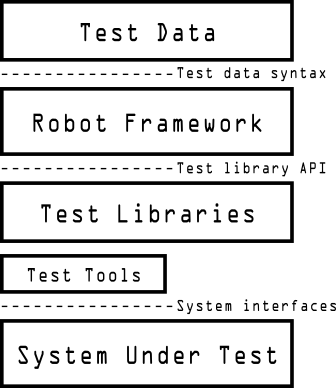
\includegraphics[width=0.4\textwidth]{assets/robot-arkkitehtuuri.png}
      \caption{Robot framework alustan arkkitehtuuri}
      \label{fig:robot-architecture}
    \end{figure}

    Robot frameworkillä rakennettuja testitapauksia voidaan ajaa komentoriviltä robot komennolla.
    Testitapauksien ajaminen tulostaa komentoriville yksinkertaisen raportin testitapauksen onnistumisesta ja lisäksi tallettaa varsin yksityiskohtaisen ja selkeän testitaportin ajetuille testitapauksille.
    Testiraportit ovat erittäin hyvin tehtyjä ja html-pohjaisia, joka tarkoittaa että ne voidaan helposti integroida osaksi jatkuvan integraation koontiputkia.

    Yhtenä heikkoutena Robot frameworkissa on tuen puuttuminen ohjelmistokieliperustaisissa testikehyksissä löytyville kontrollirakenteille, joita esiintyy esimerkiksi yksikkötestaukseen tarkoitetuissa testikehyksissä.
    Robot framework on selkeästi vain hyväksymistestauksen testitapauksien rakentamista varten tarkoitettu testialusta ja siinä se on erinomainen vaihtoehto testitapauksien rakentamiseen.

  \subsection{Selenium} \label{ch:08_selenium}

    % TODO: Kirjoita tämä kappale

    \begin{itemize}
      \item Mikä se on?
      \item Mihin sitä käytetään?
      \item Mitä hyötyjä siitä saadaan?
      \item Sisäinen rakenne / yksityiskohtainen esittely
      \item (Mitä heikkouksia siinä on?)
      \item Yhden lauseen yhteenveto
    \end{itemize}

  \subsection{Xvfb} \label{ch:08_xvfb}

    % TODO: Kirjoita tämä kappale

    \begin{itemize}
      \item Mikä se on?
      \item Mihin sitä käytetään?
      \item Mitä hyötyjä siitä saadaan?
      \item Sisäinen rakenne / yksityiskohtainen esittely
      \item (Mitä heikkouksia siinä on?)
      \item Yhden lauseen yhteenveto
    \end{itemize}

  \subsection{GoCD} \label{ch:08_gocd}

    % TODO: Kirjoita tämä kappale

    \begin{itemize}
      \item Mikä se on?
      \item Mihin sitä käytetään?
      \item Mitä hyötyjä siitä saadaan?
      \item Sisäinen rakenne / yksityiskohtainen esittely
      \item (Mitä heikkouksia siinä on?)
      \item Yhden lauseen yhteenveto
    \end{itemize}

  \subsection{Docker} \label{ch:08_docker}

    % TODO: Kirjoita tämä kappale

    \begin{itemize}
      \item Mikä se on?
      \item Mihin sitä käytetään?
      \item Mitä hyötyjä siitä saadaan?
      \item Sisäinen rakenne / yksityiskohtainen esittely
      \item (Mitä heikkouksia siinä on?)
      \item Yhden lauseen yhteenveto
    \end{itemize}

\section{Testitapauksien määrittäminen} \label{ch:08_testitapauksien_maarittaminen}

  Testitapaus on testiautomaation näkökulmasta, määritelty toimenpiteiden, ehtojen ja muuttujien joukko, joka suorittamalla voidaan verifioida ominaisuus tai toiminnallisuus ohjelmistosta.
  Testitapauksiin liittyy oleellisesti testikokoelman käsite, joka tarkoittaa samaan kontekstiin kuuluvista testitapauksista muodostettua joukkoa.
  Tässä diplomityössä keskitettyyn hyväksymistestaukseen liittyen testitapaukset kirjoitetaan usein käyttötapauksien muodossa.
  Lisäksi hyväksymistestauksen priorisoimiseen painotetun verkon avulla on suositeltavaa suunnitella ja rakentaa testitapaukset näkymä ja siirtymäperusteisesti, jotta matemaattisia verkkoja voidaan kunnolla hyödyntää.

  Testitapauksen perusformaatti koostuu lähtötilanteesta, laukaisijasta ja verifikaatiosta.
  Lähtötilanteessa oletetaan jotakin ja seuraavassa vaiheessa seurataan kun jokin ehto tapahtuu, jonka jälkeen voidaan tarkistaa seuraus ja verifioida onko se oletuksen mukainen.
  Testitapauksien yleisiä tavoitteita ovat: yksinkertaisuus, läpinäkyvyys, käyttäjätietoisuus, epätoistuvuus, olettamattomuus, kattavuus, tunnistettavuus, jälkensä puhdistava, toistettava, syvyyttömyys ja atomisuus.

  \noindent\begin{minipage}{\linewidth}
  \renewcommand{\lstlistingname}{Koodi}
  \lstinputlisting[
    caption={Esimerkki testitapauksesta Robot frameworkillä},
    label=code:robot-framework-testitapaus,
    numbers=left
  ]{assets/robot-framework-testitapaus.robot}
  \end{minipage}

  Robot Frameworkin perustaja on kirjoittanut laajan ohjeistuksen siitä, miten Robot Frameworkiä käyttäen luodaan hyviä testitapauksia \parencite{klarck_how-to-write-good-test-cases_2019}.
  Klärckin ohjeistuksen pohjalta on huomioitavaa erityisesti testikokoelmien, testitapauksien ja avainsanojen nimeäminen jonka kuuluisi olla selkeää, kuvaavaa ja ytimekästä.
  Dokumentaation määrää testitapauksissa tulisi rajoittaa, sillä hyvin kirjoitetut testitapaukset ovat Robot frameworkiä käyttäen selkeitä jo sellaisenaan.
  Dokumentaatiota kuuluisi lisätä lähinnä vain testikokoelmiin yleisellä tasolla.
  Testikokoelmat kuuluisi sisältää vain toisiinsa liittyviä testejä ja testitapauksien sekä avainsanojen tulisi olla sellaisinaan selkeästi ymmärrettäviä.
  Muuttujien käyttöä suositellaan kapsuloimaan pitkiä ja kompleksisia arvoja, mutta arvojen syöttäminen ja palauttaminen muuttujia hyödyntäen tulisi pitää pois testitapauksien tasolta.

\section{Priorisointiongelma} \label{ch:08_priorisointiongelma}

  Testitapauksien priorisointi on kustannussyistä tai resurssien optimoinnin kannalta erittäin tärkeää.
  Ohjelmistotestauksessa on hyvä tiedostaa, että ohjelmistotuotetta ei usein voida testata täydellisesti, joka nostaa esiin tarpeen tärkeimpien testitapauksien löytämisestä.
  Priorisoinnin toutettamisen tärkeys korostuu erityisesti silloin kun kohdejärjestelmä on kompleksinen ja toimminallisia ominaisuuksia on paljon.

  Priorisoinnista saatavia hyötyjä:
  \begin{itemize}
    \item Tärkeät ongelmat löydetään aikaisin
    \item Testitapauksien suorittamisen järjestäminen
    \item Epäoleelliset testitapaukset voidaan jättää toteuttamatta
    \item Kustannuksia ja resursseja säästyy
    \item Käytännönläheisyys
    \item Korkean prioriteetin testitapauksiin voidaan käyttää huolellista suunnittelua
  \end{itemize}

  % TODO: Lisää tekstiä tähän kappaleeseen. Eheyden kannalta tärkeä kappale!
  <TODO: kirjoita tähän lisää tekstiä...>

  Priorisointiongelmaan on olemassa useita erilaisia lähestymistapoja ja menetelmiä, kuten esimerkiksi heuristinen priorisointi tai MoSCoW menetelmä.
  Tässä diplomityössä priorisointiin käytetään kuitenkin matemaattista painotettuihin verkkoihin perustuvaa lähestysmistapaa, joka on uudenlainen tämän diplomityön tuotteena kehittynyt menetelmä priorisointiongelman ratkaisemiseen.

\chapter{Priorisointi painotetun verkon avulla} \label{ch:09_priorisointi_painotetun_verkon_avulla}
  Tässä luvussa käsitellään ensin työhön keskeisesti kuuluvan verkkoteorian perusteita ja käydään huolellisesti läpi niistä tässä työssä käytettävät osat.
Työssä sovelletaan erityisesti verkkoteorian painotettua verkkoa sekä siihen liittyviä käsitteitä.
Verkkoteoria itsessään on osa diskeettiä matematiikkaa.

Verkkoteorian jälkeen esitetään vaiheittain työn tuloksena kehitetty priorisointimenetelmä.
Priorisointia varten esitetään harkintaa käyttäen valitut priorisointiin vaikuttavat muuttujat, niitä käyttävät painofunktiot, verkon rakentaminen ja karsiminen sekä verkon ja testitapauksien yhteys.
Lisäksi käydään läpi, miten menetelmää käyttäen tuotetun painotetun verkon sisältämää informaatiota voidaan hyödyntää prioriteeteiltaan tärkeimmän polun löytämiseen Dijkstran algoritmin avulla.

\section{Matemaattisten verkkojen tarkoitus} \label{ch:09_matemaattisten_verkkojen_tarkoitus}

  Matemaattisten verkkojen tarkoituksena on mallintaa parittaisia riippuvuuksia verkkomaisessa objektijoukossa.
  Verkkoteoriassa peruskäsitteitä ovat itse verkko eli graafi, joka muodostuu solmuista ja solmujen välisiä riippuvuuksia esittävistä kaarista tai nuolista.
  Verkkoteorialla on lukuisia käytännön sovellutuksia. Verkkoteoriaa sovelletaan muun muassa tietokonetieteissä, kielitieteissä, fysiikan ja kemian sovellutuksissa, sosiaalisissa tieteissä sekä biologiassa.
  Alun perin verkkoteorian katsotaan syntyneen 1700-luvulla esiintyneestä, niin sanotusta Königsbergin siltaongelmasta, johon Leonhard Euler esitti todistuksensa \parencite{graph_theory_concepts_1}.

  Matemaattisten verkkojen käyttöön päädyttiin tässä työssä siksi, että niiden avulla on hyväksymistestauksen kohteena oleva käyttöliittymä mahdollista mallintaa verkoksi.
  Käyttöliittymän verkkomuotoiseen esitykseen voidaan vielä lisätä painot, jotka tässä tapauksessa kuvaavat prioriteetteja, mahdollistaen testikokoelmien priorisoinnin.

\section{Perusmerkinnät ja käsitteet} \label{ch:09_perusmerkinnat_ja_kasitteet}

  Verkkoteoriaa käsittelevässä kirjallisuudessa \parencite{graph_theory_concepts_1}\parencite{graph_theory_concepts_2}\parencite{graph_theory_concepts_3} käytetään muun muassa seuraavia perusmerkintöjä ja käsitteitä:

  \begin{itemize}
    \item \textbf{Solmujoukko} \(V = \{v_a, v_b, v_c\}\) on joukko joka sisältää solmut \(v_a\), \(v_b\) ja \(v_c\).
    \item \textbf{Kaarijoukko} \(E = \{e_{ab}, e_{bc}, e_{ac}\}\) on joukko joka sisältää kaaret \(e_{ab}\), \(e_{bc}\) ja \(e_{ac}\).
    \item \textbf{Verkko} \(G = V(G) \cup E(G)\) on joukko joka sisältää solmujoukon \(V(G)\) ja kaarijoukon \(E(G)\).
    \item \textbf{Aliverkko} \(G_s \subset G\) on verkko \(G_s\) joka koostuu osasta verkon \(G\) solmuja ja kaaria.
    \item \textbf{Polku} \(P = \{v_a, v_b, ..., v_n \: | \: v_a \rightarrow v_n\}\) on solmujono, jota pitkin voidaan kulkea solmusta \(v_a\) solmuun \(v_n\).
    \item \textbf{Sykli} \(C = \{v_a, ..., v_n,..., v_a \: | \: v_a \rightarrow v_a\}\) on sellainen polku, jonka aloitussolmu \(v_a\) ja lopetussolmu \(v_a\) ovat sama solmu siten, että polun jokaista kaarta kuljetaan vain kerran.
    \item \textbf{Verkon yhtenäisyys} \(\forall \: v_a \neq v_b \: \exists \: P_{ab}\) tarkoittaa sitä, että \(v_a \rightarrow v_b\), jokaiselle solmuparille on olemassa niitä yhdistävä polku.
    \item \textbf{Solmun asteluku} \(d_G(v_a)\) on solmuun \(v_a\) liittyvien kaarten lukumäärä.
    \item \textbf{Eristetty solmu} on solmu \(v_a\), jonka asteluku on nolla, eli \(d_G(v_a) = 0\).
    \item \textbf{Silta} on solmujen \(v_a\) ja \(v_b\) välinen kaari \(e_{ab}\) siten, että \(d_G(v_a) = 1\) ja \(d_G(v_b) = 1\).
    \item \textbf{Silmukka} on kaari, jonka aloitus- ja lopetussolmu  ovat sama solmu, eli \(v_a \rightarrow v_a\).
  \end{itemize}

\section{Priorisointiin vaikuttavat muuttujat} \label{ch:10_priorisointiin_vaikuttavat_muuttujat}

  Näkymä- ja siirtymäperustaiseen priorisointiin vaikuttavat monet eri asiat, joista osa kasvattaa prioriteettia ja osa laskee sitä.
  Prioriteettia kasvattava muuttuja on esimerkiksi liiketoiminnallinen arvo, ja laskeva muuttuja on esimerkiksi projektin muutosherkkyys, joka voi johtaa nyt toteutettavien testitapauksien vanhentumiseen tulevaisuudessa.
  Muuttujat, niiden etumerkit ja arviointiasteikot esitetään kokonaisuudessaan taulukossa \ref{tab:priorisointiin_vaikuttavat_muuttujat}.
  Muuttujat ovat kuitenkin hyvin kontekstiriippuvaisia, joten yleispätevää ja kaikkiin tilanteisiin soveltuvaa listaa muuttujista on hankala antaa.
  Kontekstiriippuvaisuuden takia muuttujiin ja myöhemmin esitettäviin painofunktioihin on varattu paikka omille lisämuuttujille.
  Prioriteetin määrittäminen on tässä menetelmässä lineaarista, eli prioriteetti määräytyy sen osiensa summana laskukaavalla, joka myöhemmin esitetään.
  Toisin sanoen epälineaarisuutta, eli sellaista tilannetta, jossa prioriteettia ei syystä tai toisesta voitaisi ilmoittaa yksinkertaisesti osiensa summana, ei tässä menetelmässä oteta huomioon.

  \begin{table}[H]
    \caption{Näkymä- ja siirtymäperustaiseen priorisointiin vaikuttavat muuttujat}
    \label{tab:priorisointiin_vaikuttavat_muuttujat}
    \centering
    \begin{tabular}{l|l|l|l} \hline
    \(m\) & \textbf{Muuttuja} & \textbf{Etumerkki} & \textbf{Asteikko} \\ \hline
    \textbf{1} & Liiketoiminnallinen arvo & \(+\) & 1 - 10 \\
    \textbf{2} & Liiketoiminnallinen visio & \(+\) & 1 - 10 \\
    \textbf{3} & Negatiivinen käyttäjäpalaute & \(+\) & 1 - 5 \\
    \textbf{4} & Käyttötapauksien määrä & \(+\) & 10 \(\cdot\) suhde  \\
    \textbf{5} & Siirtymien määrä & \(+\) & 10 \(\cdot\) suhde  \\
    \textbf{6} & Positiivinen käyttäjäpalaute & \(-\) & 1 - 5  \\
    \textbf{7} & Muutosherkkyys & \(-\) & 1 - 10  \\
    \textbf{8} & Toteuttamisen kompleksisuus & \(-\) & 1 - 5  \\
    \textbf{9} & Toteutuksen virheherkkyys & \(-\) & 1 - 5  \\
    \textbf{10} & Omat lisämuuttujat & \(\pm\) & 1 - 10 \\ \hline
    \end{tabular}
  \end{table}

  Tässä diplomityössä esiteltävää priorisointimenetelmää varten jokainen priorisointiin vaikuttava muuttuja arvioidaan asteikolla 1-10, paria poikkeusta lukuun ottamatta.
  Numeerisella asteikolla on tarkoitus antaa korkea numero, jos muuttuja on prioriteetiltaan tärkeä kyseisen näkymän, eli verkon solmun kohdalla.
  Jos jokin muuttuja ei ole kelpoinen siinä kontekstissa, jossa menetelmää yritetään hyödyntää, tulee muuttujan arvo asettaa nollaksi, jolloin se sivuutetaan myöhemmin esitettävässä painofunktiossa.

  Poikkeukselliset muuttujat ovat käyttötapauksien määrä ja siirtymien määrä, joissa numeerisen asteikon sijaan käytetään kyseisten muuttujien määrää suhteessa koko verkkoon.
  Esimerkiksi siirtymien määrää ilmaiseva suhde määritetään laskemalla solmun asteluku \(d_G(v)\), eli solmuun liittyneiden kaarien määrä, jaettuna kaikilla verkossa olevien kaarien määrällä.
  Lisäksi siirtymien määrän suhde vielä kerrotaan luvulla 10, jotta se saadaan skaalautumaan muiden muuttujien kanssa samalle tasolle.

\section{Painofunktiot priorisointiin} \label{ch:10_painofunktiot_priorisointiin}

  Painofunktioiden määrittäminen on tärkeä osa painotetun verkon avulla tehtävää priorisointia, sillä niiden avulla määritetään verkon solmujen ja kaarien prioriteetit.
  Tavanomaisesti numeerisen prioriteetin usein mielletään olevan korkea, jos priorisoitu muuttuja on tärkeä.
  Painotettujen verkkojen tapauksessa on kuitenkin järkevää vaihtaa numeerisen prioriteetin suuntaa, jotta painotettuun verkkoon sovellettavat lyhimmän polun algoritmit toimisivat halutulla tavalla, eli etsien prioriteetiltaan tärkeitä polkuja.

  Ennen prioriteetin suunnanvaihtoa, voidaan kokonaisprioriteetti yksittäiselle solmulle eli näkymälle määrittää kaavalla

  \begin{equation} \label{eq:5_4_1}
    p(v) = \sum\limits_{i=1}^{5} m_i - \sum\limits_{j=6}^{9} m_j \pm m_{10}\text{,}
  \end{equation}

  jossa kokonaisprioriteettia solmulle \(v\) kuvataan funktiona \(p(v)\). Siinä kokonaisprioriteetin arvo määräytyy lineaarisesti osiensa \(m_k\) summana siten, että \(1 \leq k \geq 10\).
  Toisin sanoen prioriteettiin vaikuttavia erilaisia muuttujia on kaavassa yhteensä kymmenen.
  Jokainen kaavassa esiintyvä muuttuja sisältää etumerkin aiemmin esitetyn taulukon \ref{tab:priorisointiin_vaikuttavat_muuttujat} mukaisesti.
  Kaavassa esitetään ensin kokonaisprioriteettiin positiivisesti vaikuttavien muuttujien summa, joka sisältää etumerkiltään positiiviset muuttujat väliltä \(1 \leq i \geq 5\).
  Samalla periaatteella kaavassa esitetään seuraavaksi negatiivisesti vaikuttavat muuttujat väliltä \(6 \leq j \geq 9\), jotka lasketaan ensin yhteen ja vähennetään sitten yhteisesti etumerkillään negatiivisena edellisestä summasta.
  Lopuksi kaavassa on esitetty vielä viimeinen muuttuja \(m_{10}\), joka tarkoittaa taulukon \ref{tab:priorisointiin_vaikuttavat_muuttujat} mukaisesti omaa lisämuuttujaa tai lisämuuttujia, joiden etumerkki voi olla joko positiivinen tai negatiivinen.
  Lisämuuttujien sisällyttämisellä kaavaan on tarkoitus mahdollistaa ja selventää kokonaisprioriteetin laskeminen erilaisissa kontekstiriippuvaisissa tilanteissa, sekä osittain myös rohkaista kaikkien prioriteettiin vaikuttavien muuttujien evaluointiin ja muokkaamiseen kontekstista riippuen.

  Prioriteetin suunnan vaihtamisen suuresta pieneen, säilyttäen kuitenkin prioriteetin sisältämän informaation, voi hoitaa käänteislukujen avulla.
  Ennen käänteisluvuksi muuttamista, prioriteettiin vaikuttavien muuttujien yhteenlaskettu summa voi olla ongelmallisesti negatiivinen tai nolla.
  Negatiiviset arvot eivät ole painotetun verkon kannalta erityisen järkeviä, sillä tässä diplomityössä hyödynnettävää Dijkstran algoritmia ei voida käyttää negatiivisien painojen kanssa.
  Dijkstran algoritmin toiminta nollan tapauksessa voi myös kuulostaa epäilyttävältä, kuten esimerkiksi tilanne, jossa painotetun verkon kaikki painot olisivat nollia.
  Dijkstran algoritmin tapauksessa tällainen verkko on kuitenkin sallittu, koska silloin lyhimmän polun ratkaisu on verkon kaikki solmut.
  Lyhimmän polun ongelman erityisvaatimusten lisäksi käänteislukua varten nolla on huono arvo siksi, että sille ei ole olemassa lainkaan käänteislukua.
  Tämä johtuu siitä, että jos nollalle yrittäisi etsiä käänteislukua, tulisi eteen nollalla jakaminen, jota ei voi tehdä.
  Nämä molemmat ongelmatapaukset voidaan kuitenkin painofunktioissa ratkaista siten, että käänteisfunktiota ei etsitä, vaan korvataan painofunktion tulos yhdellä.

  Painofunktio yksittäiselle solmulle \(v\), eli näkymälle, saadaan solmun kokonaisprioriteetin \(p(v)\) käänteislukuna kaavalla

  \begin{equation} \label{eq:5_4_2}
    \alpha(v) = \begin{cases}
      p^{-1}(v) & p(v) > 0 \\
      1 & p(v) \leq 0
    \end{cases}
    \text{,}
  \end{equation}

  jossa solmun \(v\) käännettyä kokonaisprioriteettia kuvataan funktiona \(\alpha(v)\).
  Solmun kokonaisprioriteettia vastaava käänteisluku etsitään vain siinä tapauksessa, jos kokonaisprioriteetti on suurempi kuin nolla.
  Jos vastaan tulee tilanne, jossa kokonaisprioriteetti olisi negatiivinen tai yhtä suuri kuin nolla, ei käänteislukua yritetä ottaa, vaan tulos korvataan suoraan käännettyjen prioriteettien alhaisimmalla arvolla, eli luvulla yksi.
  Toisin sanoen painofunktiosta saatava numeerinen arvo tarkoittaa käytännössä sitä, että mitä pienempi se on, sitä korkeampaa prioriteettia se edustaa.

  Painofunktio yksittäiselle kaarelle \(e_{ab}\), eli solmuja \(v_a\) ja \(v_b\) yhdistävälle käyttöliittymän näkymien väliselle siirtymälle, saadaan kaavalla

  \begin{equation} \label{eq:5_4_3}
    \beta(e_{ab}) = \begin{cases}
      [p(v_a) + p(v_b)]^{-1} & p(v_a) + p(v_b) > 0 \\
      1 & p(v_a) + p(v_b) \leq 0
    \end{cases}
    \text{,}
  \end{equation}

  jossa kaaren \(e_{ab}\) käännettyä kokonaisprioriteettia kuvataan funktiona \(\beta(e_{ab})\). Kaaren painofunktiota varten pitää kuitenkin huomioida, että sen kokonaisprioriteetti on kaaren päätepisteiden, eli aloitus- ja lopetussolmujen kokonaisprioriteetin summa \(p(v_a) + p(v_b)\).
  Kaaren kokonaisprioriteetti pitää siis laskea ennen käänteisluvuksi muuttamista.
  Kaaren painofunktioon \(\beta(e)\) pätevät samat reunaehdot kuin yksittäisen solmun painofunktioon \(\alpha(v)\).

\section{Verkon rakentaminen} \label{ch:10_verkon_rakentaminen}

  Tässä diplomityössä on aiemmin kerrottu näkymä- ja siirtymäperusteisesta testiautomaation toteuttamisesta ja priorisoinnista.
  Painotetun verkon rakentamista varten tulee tarvittavat näkymät ja niiden väliset siirtymät muodostaa testauskohteen käyttöliittymästä.
  Web-sovelluksen käyttöliittymän näkymiä ovat muun muassa sivut, sivujen sisältämät säiliö-elementit ja dialogit.
  Jos käyttöliittymän näkymä sisältää tilan, eli kyseinen näkymä muuttuu käyttäjän tekemien toimenpiteiden perusteella, käsitellään kyseinen tilallinen näkymä painotetussa verkossa kuitenkin yhtenä solmuna.
  Tällaisessa tapauksessa menetelmän käyttö priorisoi kyseisen näkymän, joka periaatteessa vastaa sellaista testikokoelmaa, johon rakennettaisiin testitapaukset eri tilanteita varten.
  Siirtymät ovat usein sivujen välisiä linkkejä tai vaihtoehtoisesti jotakin sellaista toiminnallisuutta, joka muuttaa nykyisen näkymän tai osan siitä toiseksi näkymäksi.

  Seuraavassa taulukossa \ref{tab:esimerkki_verkon_priorisointi_muuttujat} on esitetty kuvitteellisen web-sovelluksen mukainen näkymien ja siirtymien mukaan laadittu esimerkki.
  Taulukossa esitetään näkymät kirjautumisnäkymästä ohjenäkymään, ja jokaisen näkymän siirtymät eli yhteydet toisiin näkymiin.
  Näkymät ja siirtymät luovat matemaattisen verkon laatimisen perusedellytykset eli datan, jonka avulla myöhemmin esitettävä painomatriisi voidaan laatia.
  Taulukossa on lisäksi esitetty jokainen näkymään liittyvä priorisointiin vaikuttava muuttuja.
  Priorisointiin vaikuttavien muuttujien arvot on laadittu subjektiivisesti kuvitteellisen esimerkin muodossa.
  Priorisointiin vaikuttavien muuttujien yhteenlaskettu prioriteetti yksittäiselle näkymälle on laskettu taulukkoon valmiiksi käyttäen aiemmin esitettyä prioriteettifunktiota \(p(n)\), jossa \(n\) tarkoittaa sitä näkymää, jolle prioriteetti lasketaan.

  \begin{table}[H]
    \caption{Esimerkkiverkon näkymät, siirtymät ja priorisointimuuttujat}
    \label{tab:esimerkki_verkon_priorisointi_muuttujat}
    \centering
    \begin{tabular}{l|l|l|l|l|l|l|l|l|l|l|l|l} \hline
    \(n\) & \textbf{Näkymä} & \textbf{Siirtymät} & \(m_1\) & \(m_2\) & \(m_3\) & \(m_4\) & \(m_5\) & \(m_6\) & \(m_7\) & \(m_8\) & \(m_9\) & \(p(n)\) \\ \hline
    \textbf{A} & Kirjautuminen & B & 10 & 10 & 0 & 2 & 1 & 0 & 5 & 5 & 5 & 8 \\
    \textbf{B} & Pelivalikko & A, C, D, G & 8 & 10 & 1 & 2 & 4 & 4 & 5 & 5 & 5 & 6 \\
    \textbf{C} & Asetukset & A, B & 4 & 6 & 5 & 2 & 2 & 2 & 5 & 5 & 5 & 2 \\
    \textbf{D} & Peli & B, E, G & 10 & 10 & 4 & 2 & 3 & 4 & 4 & 5 & 5 & 11 \\
    \textbf{E} & Tulokset & B, D, F & 6 & 8 & 0 & 2 & 3 & 5 & 5 & 4 & 5 & 2 \\
    \textbf{F} & Onnittelu & B, E & 1 & 8 & 0 & 0 & 2 & 2 & 5 & 2 & 5 & -3 \\
    \textbf{G} & Ohje & B, D & 1 & 10 & 2 & 0 & 2 & 0 & 8 & 0 & 0 & 7 \\ \hline
    \end{tabular}
  \end{table}

  Painotetun verkon rakentamisen syötteeksi täytyy käyttöliittymän näkymät ja siirtymät sekä niiden painoarvot esittää painomatriisin muodossa.
  Painoarvot saadaan aiemmin esitetyn painofunktion \(\beta(e)\) avulla.
  Painoarvo lasketaan kyseisen funktion avulla jokaiselle kahta näkymää yhdistävälle siirtymälle, eli painotetun verkon solmujen väliselle kaarelle.
  Painofunktio \(\beta(e)\) käyttää kaaren molempien päätepisteiden yhteenlaskettua prioriteettia, josta käänteisluku otetaan.
  Näin saadaan laskettua kaarelle sellainen painoarvo, joka tarkoittaa painotetussa verkossa siirtymän näkymiin sidottua prioriteettia.
  Esimerkkinä voidaan laskea taulukon \ref{tab:esimerkki_verkon_priorisointi_muuttujat} mukaisten näkymien \(v_a\) ja \(v_b\) välisen siirtymän, eli kaaren \(e_{ab}\) painoarvo \(\beta(e_{ab})\) seuraavalla laskutoimituksella

  \begin{equation} \label{eq:5_5_1}
    \beta(e_{ab}) = [p(v_a) + p(v_b)]^{-1} = (8 + 6)^{-1} = \frac{1}{14} \approx 0.071
    \text{.}
  \end{equation}

  Painofunktioiden lisäksi painotetun verkon esittämistä varten tarvitaan painomatriiseja.
  Painomatriisin avulla voidaan rakentaa matemaattinen painotettu verkko, joka kuvaa näkymiä ja siirtymiä sekä niiden prioriteetteja.
  Painomatriiseissa tulee lähes väistämättä esiin tilanne, jossa pitäisi määrittää painoarvo olemattomalle silmukalle eli kaarelle, jonka aloitussolmu ja lopetussolmu ovat sama solmu itsessään, mutta kaarta ei ole olemassa.
  Tällaisissa tapauksissa, tilanteesta riippuen, painomatriiseihin merkitään usein \(0\), \(\infty\) tai \(-\) \parencite{graph_theory_concepts_1}.
  Tässä diplomityössä esitettävän menetelmän painomatriiseissa solmuun itseensä johtuvan kaaren eli silmukan painoksi merkitään aina \(-\), koska käyttöliittymän näkymästä siirtymät itseensä ei tässä menetelmässä käsitellä varsinaisina siirtyminä.
  Tämän lisäksi luonnollisesti jokainen sellainen solmupari, jolla ei ole niitä yhdistävää kaarta, merkitään painomatriisiin käyttäen \(-\) merkintää.
  Sellaisien siirtymien toiminnallisuuden testaaminen on tarkoitus kattaa näkymän mukaisen testikokelman testitapauksissa ja ne tulevat priorisoiduiksi näkymä- ja siirtymäperusteisesti.
  Painotetun verkon kaaret voivat verkkoteorian mukaan olla suunnattuja tai suuntaamattomia \parencite{graph_theory_concepts_1}.
  Tässä esimerkkitapauksessa jokainen siirtymä näkymien välillä on suuntaamaton, eli toisin sanoen käyttöliittymässä kaksisuuntainen, ja se priorisoidaan sen mukaisesti.
  Painomatriisissa suuntaamattomien kaarien johdosta voidaan huomata, että painomatriisin diagonaalin erottamat puoliskot ovat toistensa peilikuvia.
  Painomatriisi taulukon \ref{tab:esimerkki_verkon_priorisointi_muuttujat} mukaiselle esimerkille ja siitä lasketuille painoarvoille on pyöristettynä kolmen desimaalin tarkkuudelle seuraavanlainen:

  \begin{equation} \label{eq:5_5_2}
    M_G \approx
    \bordermatrix{
      G   & v_a   & v_b   & v_c   & v_d   & v_e   & v_f   & v_g   \cr
      v_a & -     & 0.071 & 0.100 & -     & -     & -     & -     \cr
      v_b & 0.071 & -     & 0.125 & 0.059 & 0.125 & 0.333 & 1.000 \cr
      v_c & 0.100 & 0.125 & -     & -     & -     & -     & -     \cr
      v_d & -     & 0.059 & -     & -     & 0.077 & -     & 0.250 \cr
      v_e & -     & 0.125 & -     & 0.077 & -     & 1.000 & -     \cr
      v_f & -     & 0.333 & -     & -     & 1.000 & -     & -     \cr
      v_g & -     & 1.000 & -     & 0.250 & -     & -     & -     \cr
    }
    \text{.}
  \end{equation}

  Painomatriisin määrittämisen jälkeen voidaan edetä painotetun verkon kuvaamiseen, jossa piirretään jokainen erilaista käyttöliittymän näkymää vastaava, esimerkkidatan mukainen solmu, ja niiden välisiä siirtymiä kuvaavat yhteydet eli kaaret.
  Kaarien yhteyteen lisätään painomatriisista kaaren prioriteettia kuvaava painoarvo.
  Seuraavassa on esitetty painomatriisia vastaava painotetun verkon kuvaaja sellaisena kuin se on ennen siihen tehtäviä prioriteettileikkauksia.
  Toisin sanoen kyseinen painotetun verkon kuvaaja on lähtötilanne, josta priorisointi aloitetaan.
  Priorisoimista varten tehtävien leikkauksien tekeminen niitä varten kehitetyllä toistettavalla karsimisalgoritmilla esitetään myöhemmin omassa kappaleessaan.

  \begin{figure}[H]
    \centering
    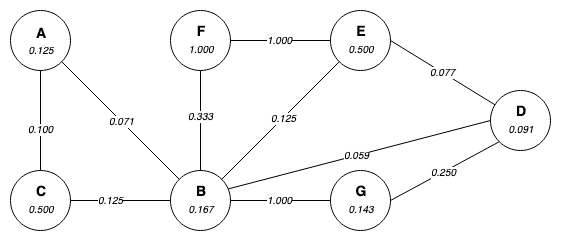
\includegraphics[width=0.8\textwidth]{assets/painotettu-verkko-ennen.png}
    \caption{Esimerkki painotetusta verkosta ennen leikkauksia}
    \label{fig:painotettu-verkko-ennen}
  \end{figure}

  Perinteisesti painotetuissa verkoissa ei esitetä yksittäisiä solmupainoja, vaan painotetun verkon painoilla tarkoitetaan solmujen välisien kaarien painoarvoja.
  Tässä diplomityössä kehitettyä menetelmää käytettäessä edellä esitettyyn painotettuun verkkoon on kuitenkin lisätty painomatriisin sisältämän informaation lisäksi painofunktion \(\alpha(v)\) avulla lasketut yksittäisten solmujen eli näkymien painoarvot.
  Esimerkkinä voidaan laskea taulukon \ref{tab:esimerkki_verkon_priorisointi_muuttujat} mukaisen näkymän eli solmun \(v_a\) painoarvo \(\alpha(v_a)\) seuraavalla laskutoimituksella:

  \begin{equation} \label{eq:5_5_3}
    \alpha(v_a) = p^{-1}(v_a) = 8^{-1}  = 0.125
    \text{.}
  \end{equation}

  Yksittäisten solmujen prioriteettia kuvaavat painoarvot ovat erittäin merkittäviä ja hyödyllisiä, sillä niiden avulla voidaan järjestää itse solmut eli näkymät prioriteettien mukaiseen järjestykseen.
  Tämän lisäksi solmujen prioriteettien avulla voidaan verkkoon soveltaa muun muassa lyhimmän polun ratkaisemiseen kehitettyjä algoritmeja, kuten myöhemmin Dijkstran algoritmin osalta esitetään omassa kappaleessaan.

\section{Verkon karsiminen} \label{ch:10_verkon_karsiminen}

  Painotetun verkon karsiminen, eli sen kaarien leikkaaminen, on yksi prioriteeillä painotetun verkon erittäin tärkeistä ominaisuuksista.
  Verkkoteorian soveltaminen prioriteettien avulla painotettuun verkkoon on erityisen hyödyllistä silloin, kun verkon kaarissa alhainen paino tarkoittaa suurta prioriteettia.
  Tässä diplomityössä verkon karsiminen tapahtuu varta vasten kehitetyllä kolmivaiheisella iteratiivisesti toistettavalla algoritmilla, jonka käyttämistä varten valitaan ensin minimirajaa vastaava kattavuus, jonka jälkeen karsiminen lopetetaan.
  Kattavuus tarkoittaa samalla myös testikattavuutta testikokoelmien näkökulmasta, sillä painotetussa verkossa jokainen solmun eli näkymän voidaan ajatella vastaavan sen mukaan kategorisoitua testikokoelmaa.

  Verkkoon tehtäviä leikkauksia varten määritettävä kattavuus \(c\) on prosentuaalinen raja sille, kuinka suuri osa verkon solmuista eli näkymistä täytyy verkkoon jäädä karsimisen jälkeen.
  Leikkauksien tekemistä suoritetaan toistuvasti niin kauan, kunnes karsittavan verkon solmujen lukumäärä on suurempi kuin kattavuuden määräämä alaraja sallii, tai jos kyseisellä iteraatiokerralla ei yksinkertaisesti enää löydy algoritmiin kuuluvilla toimenpiteillä poistettavia solmuja.
  Matemaattiseen muotoon kirjoitettuna kattavuuteen perustuva toistamisen lopettava ehto on

  \begin{equation} \label{eq:5_6_1}
    |V(G_s)| >  \frac{c}{100} \cdot |V(G)|
    \text{,}
  \end{equation}

  jossa \(|V(G_s)|\) tarkoittaa karsitun verkon solmujoukon mahtavuutta, ja vastaavasti  \(|V(G)|\) tarkoittaa alkuperäisen verkon solmujoukon mahtavuutta eli solmujen lukumäärää.
  Ehto voidaan myös ajatella yksinkertaisesti aliverkon solmujen lukumääränä, jonka täytyy olla suurempi kuin muuttujan \(c\) mukainen prosentuaalinen osuus alkuperäisen verkon solmujen lukumäärästä.
  Tässä verkon karsimisen esimerkissä kattavuutena käytetään \(c = 80\), mikä tarkoittaa esimerkkiverkon alkuperäisten solmujen määrän \(7\) karsimista määrään \(80 \cdot \frac{7}{100} = 5.6\), eli lukumäärään \(5\) asti.

  Algoritmissa on kolme erilaista toimenpidettä verkon karsimiseen.
  Toimenpiteillä on suoritusjärjestys, jonka mukaan kyseisellä iteraatiokerralla tehtävä leikkaus määräytyy.
  Jokaisella toimenpiteellä on myös oma suoritusehto, jonka täytyy täyttyä ennen kyseisen toimenpiteen suorittamista.
  Suoritusjärjestyksen ja ehtojen perusteella siirrytään toimenpiteestä toiseen yhden iteraatiokerran aikana siten, että jos esimerkiksi ensimmäistä toimenpidettä ei sen suoritusehdon mukaan voida tehdä, yritetään suorittaa toimenpiteistä seuraavaa.
  Jokaisella iteraatiokerralla suoritetaan vain yksi toimenpide, jonka jälkeen aloitetaan uusi iteraatiokierros.
  Algoritmiin sisältyvät seuraavat toimenpiteet niiden oikeaan suoritusjärjestykseen järjestettynä.

  \begin{enumerate}
    \itemsep1em
    \item \textbf{Poistetaan verkosta löytyvä eristetty solmu} eli solmu, jonka asteluku on nolla.
    Eristettyjä solmuja ei alkuperäisestä verkosta pitäisi löytyä lainkaan, vaan ne ovat seurausta eri iteraatiokerroilla tapahtuneista leikkauksista.
    Toimenpiteen suoritusehto on muotoa
      \begin{equation} \label{eq:5_6_2}
        d_G(v) = 0
        \text{,}
      \end{equation}
    jossa \(d_G(v)\) tarkoittaa astelukua  kuvaavaa funktiota solmulle \(v\).
    \item \textbf{Poistetaan verkosta löytyvä sillattu solmu} leikkaamalla siihen liittyvä kaari.
    Solmun asteluvun täytyy olla yksi ja sen painon pienempi kuin alkuperäisen verkon solmujen painojen keskiarvo.
    Toimenpiteen suoritusehto on kaksiosainen ja muotoa
      \begin{equation} \label{eq:5_6_3}
        d_G(v) = 1 \;\; \land \;\; \alpha(v) < \frac{1}{|V(G)|} \cdot \sum\limits_{v \in V(G)} \alpha(v)
        \text{,}
      \end{equation}
    jossa \(d_G(v)\) tarkoittaa astelukua solmulle \(v\) ja \(|V(G)|\) tarkoittaa alkuperäisen verkon solmujen lukumäärää sekä \(\sum\limits_{v \in V(G)} \alpha(v)\) tarkoittaa alkuperäisen verkon solmujen painoarvojen yhteenlaskettua summaa.
    \item \textbf{Poistetaan verkosta solmu, jolla on maksimia pienempi asteluku ja keskimääräistä pienempi paino.}
    Toisin sanoen poistetaan verkosta sellainen alhaisimman prioriteetin solmu, jonka asteluku on pienempi kuin solmujen astelukujen keskiarvo, ja jonka paino on pienempi kuin alkuperäisen verkon solmujen painojen keskiarvo.
    Toimenpiteen suoritusehto on kaksiosainen ja muotoa
      \begin{equation} \label{eq:5_6_4}
        d_G(v) < \text{max}\{d_G(x) | x \in V(G)\} \;\; \land \;\; \alpha(v) < \frac{1}{|V(G)|} \cdot \sum\limits_{v \in V(G)} \alpha(v)
        \text{,}
      \end{equation}
    jossa \(d_G(v)\) tarkoittaa astelukua solmulle \(v\) ja \( \text{max}\{d_G(x) | x \in V(G)\}\) tarkoittaa maksimia alkuperäisen verkon solmujen asteluvuista.
    Keskiarvon laskemiseen liittyvät merkinnät \(|V(G)|\) ja \(\sum\limits_{v \in V(G)} \alpha(v)\) ovat samat kuin edeltävässä toimenpiteessä.
  \end{enumerate}

  Tässä diplomityössä läpikäytävässä taulukon \ref{tab:esimerkki_verkon_priorisointi_muuttujat} mukaisessa verkon karsimisen esimerkissä algoritmia suoritetaan kaksi iteraatiokierrosta.
  Kahden iteraatiokierroksen jälkeen verkon solmujen määrä karsiutuu prioriteettien ja valitun kattavuuden \(c=80\) mukaisesti seitsemästä viiteen.

  \begin{figure}[H]
    \centering
    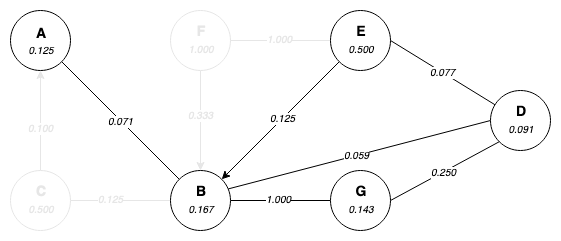
\includegraphics[width=0.8\textwidth]{assets/painotettu-verkko-jalkeen.png}
    \caption{Esimerkki painotetusta verkosta leikkauksien jälkeen}
    \label{fig:painotettu-verkko-jalkeen}
  \end{figure}

  Verkon karsimisen jälkeen voidaan huomata, että verkosta on karsiutunut pois kaksi prioriteeteiltaan alhaisinta solmua C ja F.
  Lisäksi alkuperäisestä verkosta \ref{fig:painotettu-verkko-ennen} voidaan huomata, että solmuilla C ja E olisi keskenään yhtä suuri prioriteetti, mutta asteluvuiltaan ne ovat erilaiset.
  Algoritmi toimii kyseisessä tapauksessa oikein ja karsii edellä mainituista solmuista solmun C.
  Esimerkin mukaisen solmujen karsimisen myötä voidaan todeta, että algoritmi toimii siten kuin sen kuuluukin.

\section{Dijkstran algoritmin hyödyntäminen} \label{ch:10_dijkstran_algoritmin_hyodyntaminen}

  Priorisointimenetelmän mukaan karsittuun painotettuun verkkoon on mahdollista soveltaa lyhimmän polun ongelman ratkaisemiseen kehitettyjä algoritmeja.
  Ne toimivat normaaliin tapaan etsien numeerisesti alhaisimman painoarvon polkuja, mikä kuitenkin tässä menetelmässä tarkoittaa käänteisesti korkeimman prioriteetin polkuja.
  Lyhimmän polun etsimiseen on tarkoitus valita sellaiset aloitus- ja lopetussolmut, joiden välille halutaan etsiä verkon lyhin polku.
  Lyhimmän polun löytymisen yhtenä perusedellytyksenä on verkon yhtenäisyys, joka tarkoittaa sitä, että mistä tahansa yksittäisestä verkon solmusta on löydettävissä yhteys mihin tahansa toiseen samassa verkossa olevaan solmuun.

  Prioriteeteiltaan tärkeimmän polun löytämiseksi valitaan ensin aloitussolmuksi pienimmän painoarvon solmu ja lopetussolmuksi seuraavaksi pienimmän painoarvon solmu, sekä etsitään sitten Dijkstran algoritmia hyödyntäen niiden välinen lyhin polku.
  Dijkstran algoritmin sisäinen toimintaperiaate ei ole tämän diplomityön näkökulmasta oleellista, mutta se on kuitenkin esitetty tarkemmin pseudokoodina liitteessä \ref{ch:12_liite_dijkstran_algoritmi}.
  Dijkstran algoritmi kahdelle painoltaan pienimmille, eli prioriteeteiltaan korkeimmille, solmuille antaa tuloksena kyseisiä solmuja yhdistävän polun, jonka sisältävät solmut, eli näkymät, ovat prioriteetiltaan tärkeimmät.
  Jos aloitus- ja lopetussolmut ovat vierekkäiset, eli niitä yhdistää kaari, ei polussa luonnollisesti ole kuin kaksi solmua.
  Muussa tapauksessa lyhin mahdollinen polku kertoo kaikki sellaiset käyttöliittymän näkymät, jotka ovat yhteydessä toisiinsa, ja jotka ovat yhteisesti prioriteeteiltaan tärkeimmät.
  Koska painotetun verkon painofunktiot on laadittu käänteislukuja hyödyntäen, Dijkstran algoritmi löytää painoarvoltaan matalimman, mutta prioriteetiltaan tärkeimmän polun aloitus- ja lopetussolmujen välille.
  Näin ollen saadaan helposti ja vaivattomasti tietää sellaiset solmut, eli käyttöliittymän näkymät, jotka kuuluvat prioriteetiltaan tärkeimpiin, ja joista testiautomaation rakentaminen kannattaa aloittaa.

\section{Verkon ja testitapauksien yhteys} \label{ch:10_verkon_ja_testitapauksien_yhteys}

  Priorisointi painotetun verkon avulla havainnollistaa käyttöliittymän näkymiä ja niiden välisiä siirtymiä ennen varsinaisten testitapauksien rakentamista.
  Tällaisesta painotetusta verkosta saadaan priorisoitua käyttöliittymän näkymät ja siirtymät.
  Tämä tarkoittaa käytännössä sitä, että prioriteettijärjestys saadaan määritettyä vain testikokoelmien laajuudella yksittäisten, johonkin testikokoelmaan liittyvien, testitapauksien sijaan.
  Painotetun verkon näkymät ovat suoraan yhteydessä testiautomaatiota varten rakennettaviin testikokoelmiin, jotka sisältävät kokoelman testitapauksia kyseiselle näkymälle.
  Toisin sanoen varsinaisen priorisoinnin kohteena ovat painotetun verkon näkymiä vastaavat testikokoelmat.

  Aiemmin testitapaukset ja testikokoelmat kappaleessa on esitetty niiden välistä eroa ja sitä kuinka testikokoelmat koostuvat yhteen liittyvistä testitapauksista.
  Painotetun verkon avulla tehtävää priorisointia käyttäessä on tarkoitus ajatella testiautomaation testitapauksien kategorisoimista testikokoelmiksi käyttöliittymän näkymiä vastaavalla tavalla.
  Kun käyttöliittymän näkymillä on niitä vastaavat testikokoelmat, toimii tässä diplomityössä kehitetty painotetun verkon avulla toteutattava priorisointi oikein ja siten kuin se on tarkoitettu.
  Jos testiautomaation halutaan lisätä testitapauksia tai testikokoelmia, jotka eivät ole luettavissa painotetusta verkosta, niille ei luonnollisesti ole olemassa prioriteettia ja sellaiset täytyy käsitellä ylimääräisinä, täydentävinä testitapauksina.

  Painotetun verkon kuvaamisen seurauksena, voidaan verkosta nähdä myös paljon hyödyllistä informaatiota, kuten muun muassa siinä esiintyviä sillattuja solmuja sekä syklejä.
  Sillatut solmut ovat sellaisia käyttöliittymän näkymiä, joihin käyttäjä ei kovinkaan usein päädy ja näin ollen jos niitä lopullisessa karsitussa verkossa esiintyy, ne ovat testiautomaatin rakentamisen kannalta usein vain vähän merkitseviä.
  Eristetyt solmut ovat samaan tapaan vain vähän merkitseviä kuin sillatut solmut.
  Syklit puolestaan ovat erittäin merkittävä osa painotetussa verkossa ja testiautomaation rakentamisessa, sillä ne ovat sellaisia käyttöliittymän näkymiä ja niiden välisiä siirtymiä, jotka toistuvat käyttäjälle usein käyttöliittymää käyttäessään.
  Solmujen asteluvut kertovat myös paljon solmujen merkitsevyydestä.
  Sellainen solmu jonka asteluku, eli siihen liittyvien kaarien lukumäärä on korkea, on testiautomaation rakentamisen kannalta yhtälailla erittäin merkittävä osa testiautomaatiota.

\chapter{Tulosten tarkastelu ja arviointi} \label{ch:10_tulosten_tarkastelu_ja_arviointi}
  Tässä kappaleessa esitetään yhteenveto tutkimuksen tuloksista ja evaluoidaan testausjärjestelmän ja priorisointimenetelmän toteutuksien onnistumista.
Ensin evaluoidaan diplomityössä suunnitellun ja asiakasyritykselle toteutetun testausjärjestelmän positiivisia sekä negatiivisia puolia.
Seuraavaksi evaluoidaan diplomityössä kehitetyn priorisointimenetelmän positiivisia ja negatiivisia puolia ja muun muassa pohditaan kuinka hyvin soveltuva ja toistettavissa oleva kyseinen kehitetty priorisointimenetelmä on.
Lisäksi lopussa vielä esitetään toteutuksen jälkeen esiin tulleita jatkokehitysehdotuksia testausjärjestelmälle sekä priorisointimenetelmälle.

\section{Tutkimuksen konkreettiset tulokset} \label{ch:12_tutkimuksen_konkreettiset_tulokset}

  Työn tuloksena kehitetty  web-käyttöliittymien hyväksymistestauksen automatisoimisen mahdollistava testausjärjestelmä on integroitu onnistuneesti osaksi GoCD-palvelimen avulla suoritettavaa jatkuvaa integrointia.
  Lyhyesti sanottuna testausjärjestelmän osalta konkreettinen tulos koostuu järjestelmästä, joka mahdollistaa testitapauksien luomisen Robot Framework -alustalle käyttäen Selenium-kirjastoa, Xvfb-virtualisointipalvelinta ja Docker-säiliöintiohjelmistoa.
  Testausjärjestelmän toimivuus käytännössä todettiin esimerkkitestitapauksien muodossa oikeassa ympäristössään ja testausjärjestelmän mahdollistamat ominaisuudet ovat jo itsessään oikeassa ja lopullisessa käyttöympäristössä tarvittavia.

  Web-sovelluksien näkymä- ja siirtymäperustainen painotettua verkkoa hyödyntävä priorisointimenetelmä on myös todettu toimivaksi lähestysmistavaksi priorisointiin.
  Lyhyesti sanottuna priorisointimenetelmän tuloksena on painotettuja verkkoja hyödyntävä menetelmä, jossa määritetään priorisointiin vaikuttavat muuttujat, painofunktiot, painomatriisi, prioriteetteihin perustuvien leikkauksien tekeminen ja prioriteettien löytäminen sekä lukeminen verkosta.
  Priorisointimenetelmän toimivuus käytännössä todettiin aidosta ympäristöstä yksinkertaistaen poimitusta web-sovelluksesta.
  Priorisointimenetelmän avulla todettiin, että priorisoinnin aikana toteutetut painotetun verkon leikkaukset olivat juuri niitä näkymiä, jotka vaistonvaraisesti ilman menetelmänkin käyttöä karsittaisiin.

\section{Toteutuksen evaluointi} \label{ch:12_toteutuksen_evaluointi}

  Kokonaisuutena hyväksymistestausjärjestelmän toteutus onnistui erittäin hyvin ja sen avulla on mahdollista jopa geneerisesti rakentaa web-sovelluksesta riippumattomasti hyväksymistestaus testauskohteena olevalle web-sovellukselle.

  Testausjärjestelmän positiivisia puolia ovat muun muassa Docker-säiliöinnin avulla saatava tuki myös manuaaliselle testitapauksien ajamiselle.
  Docker-säiliö, joka mahdollistaa testitapauksien ajamisen voidaan pystyttää periaatteessa mihin tahansa ympäristöön, jossa Docker on saatavilla.
  Docker-säiliöinnin avulla myös ohjelmistokehittäjät saavat valmiin hyväksymistestausjärjestelmän helposti käyttöönsä.
  Docker-säiliöinnin ja Docker-compose:n avulla rakennettu järjestelmä ei myöskään ole sidottu mihinkään ennalta määritettyyn jatkuvan integroinnin palvelimeen, joka huomattavasti helpottaa testausjärjestelmän käyttöönottoa osaksi uusia tai muuttuvaa ohjelmistotuotannon prosessia.
  Testausjärjestelmä mahdollistaa päätteettömän testauksen virtuaalisen Xfvb-näyttöpalvelimen avulla, joka on itsessään erittäin tarvittu ominaisuus jatkuvan integroinnin ja testausjärjestelmän yhdistämiseen.
  Xvfb-näyttöpalvelimen tarjoaman virtualisoinnin avulla voidaan myös uusia WebDriver rajapinnan toteuttavia verkkoselaimia lisätä päätteettömän testauksen alaisuuteen erittäin helposti ja käytännössä rajoituksitta.
  Ainoa vaatimus on, että verkkoselain on saatavilla siihen ympäristöön, jossa Xvfb-näyttöpalvelinta ajetaan.

  Testausjärjestelmässä on kuitenkin myös negatiivisia puolia, joiden osalta järjestelmän käyttö on rajattua.
  Xvfb-näyttöpalvelimen avulla voidaan päätteettömästi testata periaatteessa mitä tahansa GUI-ohjelmia, mutta rajoitteena on kuitenkin, että niiden täytyy olla saatavilla siihen ympäristöön, jossa Xvfb-näyttöpalvelinta ajetaan.
  Tämä tarkoittaa käytännössä sitä, että web-sovelluksien hyväksymistestauksen automatisoimisesta on jätettävä pois vain Window-ympäristöön saatavien verkkoselainten, kuten Internet Explorer verkkoselaimen testaaminen.
  Robot Framework takaa helpon testitapauksien luettavuuden kenelle tahansa, mutta ohjelmistokehittäjille se voi olla turhan rajatun tuntuinen.
  Ohjelmistokehittäjänä testitapauksien laatimisen yhteyteen olisi hyvä saada mahdollisuus yksikkötestauskehyksissä käytettävistä ohjelmointikielistä tuttuihin kontrollirakenteisiin, joilla testitapauksien monipuolisuutta voisi kasvattaa perinteisesti yksikkötestauksessa mahdollisien rakenteiden tasolle.
  Tämä ei kuitenkaan ole mahdollista Robot Frameissä, jossa testitapauksien laatimiseen käytetään Robot Frameworkin omaa, rajattua syntaksia.

\section{Menetelmän evaluointi} \label{ch:12_menetelman_evaluointi}

  Tässä diplomityössä kehitetyn testitapauksien priorisointimenetelmän kehittäminen onnistui erittäin hyvin ja sen käyttämisellä saavutetaan lisäarvoa etenkin keskisuurien ja suurien web-sovelluksien käyttöliittymien hyväksymistestaukseen.

  Priorisointimenetelmän positiivisia puolia ovat muun muassa sen ominaisuuksiin liittyviä asioita, kuten priorisointimenetelmän toistettavuus, ja mahdollisuus priorisoida käyttöliittymien näkymiä ja siirtymiä.
  Näkymä- ja siirtymäperusteisen priorisoinnin tarkoituksena on mahdollistaa näkymiin perustuvien testikokoelmien priorisoiminen, jolloin niiden tärkeysjärjestys saadaan selville, ja testitapauksien kirjoittaminen voidaan aloittaa prioriteetiltaan tärkeimmästä näkymästä.
  Esimerkkinä menetelmän käyttämisen tuomasta resurssien säästöstä voidaan ottaa tarkasteluun kattavuudet \(c=90\) ja \(c=50\), keskisuurelle käyttöliittymälle, jossa on yhteensä kymmenen erilaista näkymää, ja joista jokaista varten laadittaisiin esimerkin omaisesti kolme testitapausta.
  Tällaisessa tilanteessa kaikkien testitapauksien lukumääräksi tulee kolmekymmentä, joista prioriteetein painotettua verkkoa karsimalla voidaan kuitenkin tiputtaa alhaisimman prioriteetin näkymien avulla osa testitapauksista pois.
  Tämä tarkoittaa kattavuudella \(c=90\) yhden alhaisimmalla prioriteetilla painotetun näkymän jättämistä pois testauksesta, jolloin myös kolme testitapausta voidaan jättää pois toteutuksesta.
  Vastaavasti varsin häikäilemättömällä kattavuudella \(c=50\) voitaisiin jättää pois peräti viisi näkymää, mikä tarkoittaa esimerkissä viittätoista testitapausta, jotka jätettäisiin alhaisen prioriteettinsa myötä pois toteutuksesta.
  Testitapauksien toteuttamatta jättämisellä voidaan väistämättä säästää resursseja, mutta sitä ei kuitenkaan voida tehdä täysin ilman priorisointia.
  Yksi tämän menetelmän suurimmista hyödyistä tulee nimenomaan priorisoimisesta, joka mahdollistaa resurssien säästämisen edellä mainitulla tavalla.

  Menetelmän käyttäminen on tehokkainta, kun testitapaukset kategorisoidaan näkymittäin laadittuihin testikokoelmiin, sillä menetelmän kehittämisen taustalla on ollut ajatus, jossa näkymät vastaavat testikokoelmia.
  Priorisointimenetelmä perustuu matemaattisiin painotettuihin verkkoihin, jotka tuovat hyötynä lyhimmän polun ongelman ratkaisemiseen kehitettyjen algoritmien käyttämisen mahdollistamisen prioriteetiltaan korkeimpien polkujen löytämiseen kahden solmun, eli näkymän, välille.
  Lisäksi painotetun verkon ja matemaattisen lähestymistavan käyttäminen tuo hyötynä sen, että menetelmä on kohtalaisen pienellä vaivalla muunnettavissa tietokoneohjelmaksi.
  Painotettujen verkkojen käyttäminen priorisointiin pakottaa myös menetelmän käyttäjät piirtämään näkymä- ja siirtymäperusteisen painotetun verkon, jolloin se kasvattaa käyttäjien ymmärrystä testauskohteena olevasta järjestelmästä.
  Priorisointimenetelmä on tässä diplomityössä esitetyn esimerkin \ref{tab:esimerkki_verkon_priorisointi_muuttujat} mukaan todettavissa toimivaksi, ja sen avulla on suoritettu priorisointi varsinaisesta testauskohteesta yksinkertaistetulle käyttöliittymälle.

  Priorisointimenetelmässä on myös negatiivisia puolia, mutta ne eivät tässäkään tapauksessa ylitä menetelmän käytöstä saatavaa hyötyä.
  Menetelmässä esittävien toistuvien leikkauksien määrää rajaavan testikattavuuden päättäminen näkymä- ja siirtymäperusteisesti voi olla haastavaa.
  Toinen menetelmään kohdistuva kritiikki koskee menetelmän geneerisyyttä, eli käyttöönottamisen mahdollisuutta ilman muutoksia, jota on vaikea arvioida.
  Priorisointimenetelmässä käytettävät priorisointiin vaikuttavat muuttujat ovat varsin subjektiivisia ja voivat olla testausta toteuttavan tahon mukaan muuttuvia, minkä takia muuttujiin joudutaan mahdollisesti tekemään muutoksia.
  Lisäksi menetelmässä esitetty, priorisointiin vaikuttavia muuttujia hyödyntävä, funktio \(p(v)\) kokonaisprioriteetin laskemiseen ei ota muuttujien määrittämisessä mahdollisesti esiintyvää epälineaarisuutta lainkaan huomioon.
  Tämä tarkoittaa käytännössä sitä, että kokonaisprioriteetin määrittämisen on voitava olla ilmaistavissa siihen vaikuttavien osiensa summana, mikä rajoittaa menetelmän käyttöä epälineaarisissa tapauksissa.
  Negatiivista on myös se, että menetelmän käyttö on soveltuva painotettujen verkkojen luonteen mukaisesti käyttöliittymien tapauksessa soveltuvat vain kokonaisia näkymiä peilaavien testikokoelmien priorisointiin yksittäisten testitapauksien sijaan.
  Priorisointimenetelmän käyttö voi olla turhan aikaa vievää, jos käyttöliittymä on yksinkertainen.

\section{Jatkokehitysehdotukset} \label{ch:12_jatkokehitysehdotukset}

  Tämän diplomityön konkreettisina tuloksina syntyneet testausjärjestelmä ja priorisointimenetelmä ovat sellaisenaan käyttövalmiita ja toimivaksi todettuja, mutta jatkokehittelylle on luonnollisesti niissäkin sijaa.
  Testausjärjestelmän avulla toteuttava web-sovelluksien päätön hyväksymistestaus mahdollisestaan Xvfb-näyttöpalvelimen tarjoaman virtualisoinnin avulla.
  Xvfb-näyttöpalvelin on kuitenkin saatavilla vain UNIX-ympäristöihin, joka rajaa testausjärjestelmään lisättävien verkkoselaimien saatavuutta.
  Xvfb-näyttöpalvelimelle voitaisiin jatkokehityksenä etsiä monialustaisempi vaihtoehto tai ainakin vastine Window-ympäristöön, jonka avulla myös vain Window-alustalle saatavat verkkoselaimet olisi mahdollista lisätä järjestelmään.

  Yksi priorisointimenetelmään liittyvä rajoite on käyttöliittymän näkymä- ja siirtymäperustainen priorisointi, joka asettaa näkymät vastaamaan testikokoelmia.
  Jatkokehityksenä voitaisiin tutkia näkymäperusteisuuden mukaan tehtävän priorisoinnin muuntamisen mahdollisuutta käyttötapausperustaiseksi.
  Käyttötapausperustaisesti luotava verkko parhaimmillaan vastaisi oikeita käyttäjien tarpeisiin tarkoitettuja toiminallisuuksia ja voisi parantaa priorisointia.
  Priorisointimenetelmä on vahvasti matemaattinen, joka mahdollistaa sen muuntamisen kohtalaisella vaivalla tietokoneohjelmaksi.
  Priorisointimenetelmän rakentaminen automaattisen tietokoneohjelman muotoon olisi erittäin järkevää ja laskisi menetelmän käyttööottamiseen tarvittavaa vaivannäköä huomattavasti.
  Lisäksi priorisointimenetelmän näkymäpohjaisten graafien, eli painotettujen verkkojen visualisointi voitaisiin hoitaa tietokoneohjelman yhteydessä.

\chapter{Yhteenveto} \label{ch:11_yhteenveto}
  <TODO: diplomityön tavoite saavutettu....>

<TODO: tavoitteena oli xxxxxx ....>

<TODO: tutkimuskysymykseen T1 vastattiin luvussa X .....>

<TODO: tutkimuskysymykseen T2 vastattiin luvussa X .....>

<TODO: tutkimuskysymykseen T3 vastattiin luvussa X .....>

<TODO: tutkimuskysymykseen T4 vastattiin luvussa X .....>

<TODO: konkreettisista tuloksista hyötyä......>

<TODO: diplomityö loi perustan asiakasyrityksessä tarvittavan testiautomaation rakentamiseen...>
\printbibliography[heading=bibintoc]

%%%%%%%%%%%%%%%%%%%%%%%%%%%%%%%%%%%%%%%%%%%%%%%%%%%%%%%%%%%
%% Appendices
%%%%%%%%%%%%%%%%%%%%%%%%%%%%%%%%%%%%%%%%%%%%%%%%%%%%%%%%%%%
\begin{appendices}
\chapter{Esimerkki testitapauksesta Robot Framework:illä} \label{ch:12_liite_robot_testitapaus}
  \noindent\begin{minipage}{\linewidth}
\lstinputlisting[
  label=code:robot-framework-testitapaus,
  numbers=left
]{assets/robot-framework-testitapaus.robot}
\end{minipage}
\chapter{Dijkstran algoritmi pseudokoodina} \label{ch:13_liite_dijkstran_algoritmi}
  \noindent\begin{minipage}{\linewidth}
\lstinputlisting[
  label=code:dijkstras-algorithm,
  numbers=left
]{assets/dijkstras-algorithm.pseudo}
\end{minipage}
\end{appendices}
\end{document}